\documentclass[11pt,a4paper]{article}
% \documentclass[11pt,a4paper]{report}
% \documentclass[11pt,a4paper]{book}

% 设置页面
\linespread{1} %行距
\usepackage[top=1in,bottom=1in,left=1.25in,right=1.25in]{geometry}

% 使用中文xeCJK宏包
\usepackage{fontspec,xltxtra,xunicode}
\usepackage[slantfont,boldfont]{xeCJK}

% 其它需要使用的宏包
\usepackage[colorlinks,linkcolor=blue,anchorcolor=red,citecolor=green,urlcolor=blue]{hyperref} 
\usepackage{tabularx}
\usepackage{algorithm} % 算法排版
\usepackage{amsmath} % 数学符号与公式
\usepackage{amsfonts} % 数学符号与字体
\usepackage{graphics}
\usepackage{graphicx}
\usepackage{color}
\usepackage{fancyhdr} % 设置页眉页脚
\usepackage{float} % 管理浮动体
\usepackage{lineno} % 生成行号
\usepackage{listings} % 插入程序源代码l
\usepackage{multicol} % 多栏排版
\usepackage{natbib} % 管理文献引用
\usepackage{rotating} % 旋转文字,图形,表格
\usepackage{subfigure} % 排版子图形
\usepackage{titlesec} % 改变章节标题格式
\usepackage{moresize} % 更多字体大小
\usepackage{indentfirst} % 首段缩进
\usepackage{booktabs} % 使用\multicolumn
\usepackage{multirow} % 使用\multirow

% 设置页眉页脚
\renewcommand{\headrulewidth}{0.4pt} 
\renewcommand{\footrulewidth}{0.4pt}

% 设置中文字体
\setCJKmainfont[BoldFont=SimHei,ItalicFont=KaiTi]{KaiTi}
\setCJKsansfont{SimHei}
\setCJKmonofont{FangSong}
\setCJKfamilyfont{zhsong}{SimSun}
\setCJKfamilyfont{zhhei}{SimHei}
\setCJKfamilyfont{zhfs}{FangSong}
\setCJKfamilyfont{zhkai}{KaiTi}

\newcommand*{\songti}{\CJKfamily{zhsong}} % 宋体
\newcommand*{\heiti}{\CJKfamily{zhhei}} % 黑体
\newcommand*{\fangsong}{\CJKfamily{zhfs}} % 仿宋
\newcommand*{\kaishu}{\CJKfamily{zhkai}}%楷体
% 使用如下命令:{\songti 宋体} 可以临时使用宋体,类似的黑体、仿宋、楷体

% 设置英文字体
\defaultfontfeatures{Mapping=tex-text}
\setmainfont{Arial}
\setsansfont{Times New Roman} 
\setmonofont{Monaco}
\newfontfamily{\H}{SimHei}  
\newfontfamily{\E}{Arial}  

%设置listings代码宏包格式
%\lstloadlanguages{C, C++, make}
\lstset{language=C,tabsize=4,keepspaces=true,
	breakindent=22pt, 
	numbers=left,stepnumber=1,numberstyle=\tiny,
	basicstyle=\footnotesize,
	showspaces=false,
	flexiblecolumns=true,
	breaklines=true,breakautoindent=true,breakindent=4em,
	extendedchars=false,
	frame=tb,
	escapeinside=``
}

% 题目,作者,日期
\title{Libevent源码分析}
\author{Allen Xu}
\date{\E\today}

% 正文
\begin{document}
\maketitle

\section{Libevent简介}
本文档以Libevent-2.0.21版本为基础,分析其代码,始于2014年12月19日。有关windows平台的代码均不去关注,文档中出现的需要表述的代码中与windows平台有关的均已略去。

作者在分析Libevent源码时,使用的分析工具是Understand-3.1。

Libevent is an event notification library for developing scalable network servers.  The Libevent API provides a mechanism to execute a callback function when a specific event occurs on a file descriptor or after a timeout has been reached. Furthermore, Libevent also support callbacks due to signals or regular timeouts.
Libevent

Libevent is meant to replace the event loop found in event driven network servers. An application just needs to call event\_dispatch() and then add or remove events dynamically without having to change the event loop.

Currently, Libevent supports /dev/poll, kqueue(2), select(2), poll(2), epoll(4), and evports. The internal event mechanism is completely independent of the exposed event API, and a simple update of Libevent can provide new functionality without having to redesign the applications. As a result, Libevent allows for portable application development and provides the most scalable event notification mechanism available on an operating system.  Libevent can also be used for multithreaded programs.  Libevent should compile on Linux, *BSD, Mac OS X, Solaris and, Windows.

usage Standard usage

Every program that uses Libevent must inclurde the <event2/event.h> header, and pass the -levent flag to the linker.  (You can instead link -levent\_core if you only want the main event and buffered IO-based code, and don't want to link any protocol code.)

setup Library setup

Before you call any other Libevent functions, you need to set up the library.  If you're going to use Libevent from multiple threads in a multithreaded application, you need to initialize thread support -- typically by using evthread\_use\_pthreads() or evthread\_use\_windows\_threads().  See <event2/thread.h> for more information.

This is also the point where you can replace Libevent's memory management functions with event\_set\_mem\_functions, and enable debug mode with event\_enable\_debug\_mode().

Creating an event base

Next, you need to create an event\_base structure, using event\_base\_new() or event\_base\_new\_with\_config().  The event\_base is responsible for keeping track of which events are "pending" (that is to say, being watched to see if they become active) and which events are "active". Every event is associated with a single event\_base.

event Event notification

For each file descriptor that you wish to monitor, you must create an event structure with event\_new().  (You may also declare an event structure and call event\_assign() to initialize the members of the structure.)  To enable notification, you add the structure to the list of monitored events by calling event\_add().  The event structure must remain allocated as long as it is active, so it should generally be allocated on the heap.

loop Dispaching evets.

Finally, you call event\_base\_dispatch() to loop and dispatch events. You can also use event\_base\_loop() for more fine-grained control.

Currently, only one thread can be dispatching a given event\_base at a time.  If you want to run events in multiple threads at once, you can either have a single event\_base whose events add work to a work queue, or you can create multiple event\_base objects.

bufferevent I/O Buffers

Libevent provides a buffered I/O abstraction on top of the regular event callbacks. This abstraction is called a bufferevent. A bufferevent provides input and output buffers that get filled and drained automatically. The user of a buffered event no longer deals directly with the I/O, but instead is reading from input and writing to output buffers.

Once initialized via bufferevent\_socket\_new(), the bufferevent structure can be used repeatedly with bufferevent\_enable() and bufferevent\_disable().  Instead of reading and writing directly to a socket, you would call bufferevent\_read() and bufferevent\_write().

When read enabled the bufferevent will try to read from the file descriptor and call the read callback. The write callback is executed whenever the output buffer is drained below the write low watermark, which is 0 by default.
See <event2/bufferevent*.h> for more information.

timers Timers

Libevent can also be used to create timers that invoke a callback after a certain amount of time has expired. The evtimer\_new() function returns an event struct to use as a timer. To activate the timer, call evtimer\_add(). Timers can be deactivated by calling evtimer\_del().

摘自Libevent库中include/event2/event.h

\newpage

\section{主要数据结构}\label{S.MainStructure}
通过主要数据结构的关系,来初步观察libevent对各类event的管理框架

event结构体include/event2/event\_struct.h
\begin{lstlisting}[language=C]
struct event {
	TAILQ_ENTRY(event) ev_active_next; //激活队列
	TAILQ_ENTRY(event) ev_next; //注册事件队列
	/* for managing timeouts */
	union {
		TAILQ_ENTRY(event) ev_next_with_common_timeout;
		int min_heap_idx; //指明该event结构体在堆的位置
	} ev_timeout_pos; //仅用于定时事件处理器(event).EV_TIMEOUT类型

	//对于I/O事件,是文件描述符;对于signal事件,是信号值
	evutil_socket_t ev_fd;

	struct event_base *ev_base; //所属的event_base

	//因为信号和I/O是不能同时设置的。所以可以使用共用体以省内存
	//在低版本的Libevent,两者是分开的,不在共用体内。
	union {
	//无论是信号还是IO,都有一个TAILQ_ENTRY的队列。它用于这样的情景:
	//用户对同一个fd调用event_new多次,并且都使用了不同的回调函数。
	//每次调用event_new都会产生一个event*。这个xxx_next成员就是把这些
	//event连接起来的。
	
		/* used for io events */
		//用于IO事件
		struct {
			TAILQ_ENTRY(event) ev_io_next;
			struct timeval ev_timeout;
		} ev_io;

		/* used by signal events */
		//用于信号事件
		struct {
			TAILQ_ENTRY(event) ev_signal_next;
			short ev_ncalls; //事件就绪执行时,调用ev_callback的次数			/* Allows deletes in callback */
			short *ev_pncalls; //指针,指向次数
		} ev_signal;
	} _ev;

	short ev_events;//记录监听的事件类型 EV_READ EVTIMEOUT之类
	short ev_res;		/* result passed to event callback *///记录了当前激活事件的类型
	//libevent用于标记event信息的字段,表明其当前的状态.
	//可能值为前面的EVLIST_XXX
	short ev_flags; 

	//本event的优先级。调用event_priority_set设置
	ev_uint8_t ev_pri;
	ev_uint8_t ev_closure;
	struct timeval ev_timeout;//用于定时器,指定定时器的超时值

	/* allows us to adopt for different types of events */
	void (*ev_callback)(evutil_socket_t, short, void *arg); //回调函数
	void *ev_arg; //回调函数的参数
};
\end{lstlisting}
event结构体里面有几个TAILQ\_ENTRY队列节点类型。这里因为一个event是会同时处于多个队列之中。比如同一个文件描述符或者信号值对应的多个event会被连在一起,所有的被加入到event\_base的event也会连在一起,所有被激活的event也会被连在一起。所以会有多个QAILQ\_ENTRY。

event\_base结构体event-internal.h
\begin{lstlisting}[language=C]
struct event_base {
	/** Function pointers and other data to describe this event_base's backend. */
	const struct eventop *evsel;
	/** Pointer to backend-specific data. */
	void *evbase;

	/** List of changes to tell backend about at next dispatch.  Only used by the O(1) backends. */
	struct event_changelist changelist;

	/** Function pointers used to describe the backend that this event_base uses for signals */
	const struct eventop *evsigsel;
	/** Data to implement the common signal handelr code. */
	struct evsig_info sig;

	/** Number of virtual events */
	int virtual_event_count;
	/** Number of total events added to this event_base */
	int event_count;
	/** Number of total events active in this event_base */
	int event_count_active;

	/** Set if we should terminate the loop once we're done processing events. */
	int event_gotterm;
	/** Set if we should terminate the loop immediately */
	int event_break;
	/** Set if we should start a new instance of the loop immediately. */
	int event_continue;

	/** The currently running priority of events */
	int event_running_priority;

	/** Set if we're running the event_base_loop function, to prevent
	 * reentrant invocation. */
	int running_loop;

	/* Active event management. */
	/** An array of nactivequeues queues for active events (ones that have triggered, 
	and whose callbacks need to be called).  Low priority numbers are more important, 
	and stall higher ones.*/
	struct event_list *activequeues;
	/** The length of the activequeues array */
	int nactivequeues;

	/* common timeout logic */

	/** An array of common_timeout_list* for all of the common timeout values we know. */
	struct common_timeout_list **common_timeout_queues;
	/** The number of entries used in common_timeout_queues */
	int n_common_timeouts;
	/** The total size of common_timeout_queues. */
	int n_common_timeouts_allocated;

	/** List of defered_cb that are active.  We run these after the active events. */
	struct deferred_cb_queue defer_queue;

	/** Mapping from file descriptors to enabled (added) events */
	struct event_io_map io;

	/** Mapping from signal numbers to enabled (added) events. */
	struct event_signal_map sigmap;

	/** All events that have been enabled (added) in this event_base */
	struct event_list eventqueue;

	/** Stored timeval; used to detect when time is running backwards. */
	struct timeval event_tv;

	/** Priority queue of events with timeouts. */
	struct min_heap timeheap;

	/** Stored timeval: used to avoid calling gettimeofday/clock_gettime too often. */
	struct timeval tv_cache;

#if defined(_EVENT_HAVE_CLOCK_GETTIME) && defined(CLOCK_MONOTONIC)
	/** Difference between internal time (maybe from clock_gettime) and gettimeofday. */
	struct timeval tv_clock_diff;
	/** Second in which we last updated tv_clock_diff, in monotonic time. */
	time_t last_updated_clock_diff;
#endif

#ifndef _EVENT_DISABLE_THREAD_SUPPORT
	/* threading support */
	/** The thread currently running the event_loop for this base */
	unsigned long th_owner_id;
	/** A lock to prevent conflicting accesses to this event_base */
	void *th_base_lock;
	/** The event whose callback is executing right now */
	struct event *current_event;
	/** A condition that gets signalled when we're done processing an event with waiters on it. */
	void *current_event_cond;
	/** Number of threads blocking on current_event_cond. */
	int current_event_waiters;
#endif

	/** Flags that this base was configured with */
	enum event_base_config_flag flags;

	/* Notify main thread to wake up break, etc. */
	/** True if the base already has a pending notify, and we don't need to add any more. */
	int is_notify_pending;
	/** A socketpair used by some th_notify functions to wake up the main thread. */
	evutil_socket_t th_notify_fd[2];
	/** An event used by some th_notify functions to wake up the main thread. */
	struct event th_notify;
	/** A function used to wake up the main thread from another thread. */
	int (*th_notify_fn)(struct event_base *base);
};
\end{lstlisting}
在一个event loop中只会有一个event\_base结构体对象存在。

event\_io\_map结构体event-internal.h
\begin{lstlisting}[language=C]
#ifdef EVMAP_USE_HT
#include "ht-internal.h"
struct event_map_entry;
HT_HEAD(event_io_map, event_map_entry);
#else
#define event_io_map event_signal_map
#endif
\end{lstlisting}
其中宏EVMAP\_USE\_HT的定义在If we're on win32, then file descriptors are not nice low densely packed integers.  Instead, they are pointer-like windows handles, and we want to use a hashtable instead of an array to map fds to events.
\begin{lstlisting}[language=C]
#ifdef WIN32
#define EVMAP_USE_HT
#endif
\end{lstlisting}

event\_signal\_map结构体event-internal.h
\begin{lstlisting}[language=C]
struct event_signal_map {
	/* An array of evmap_io * or of evmap_signal *; empty entries are set to NULL. */
	void **entries;
	/* The number of entries available in entries */
	int nentries;
};
\end{lstlisting}

event管理,框架图

\begin{figure}[htb]
\begin{center}
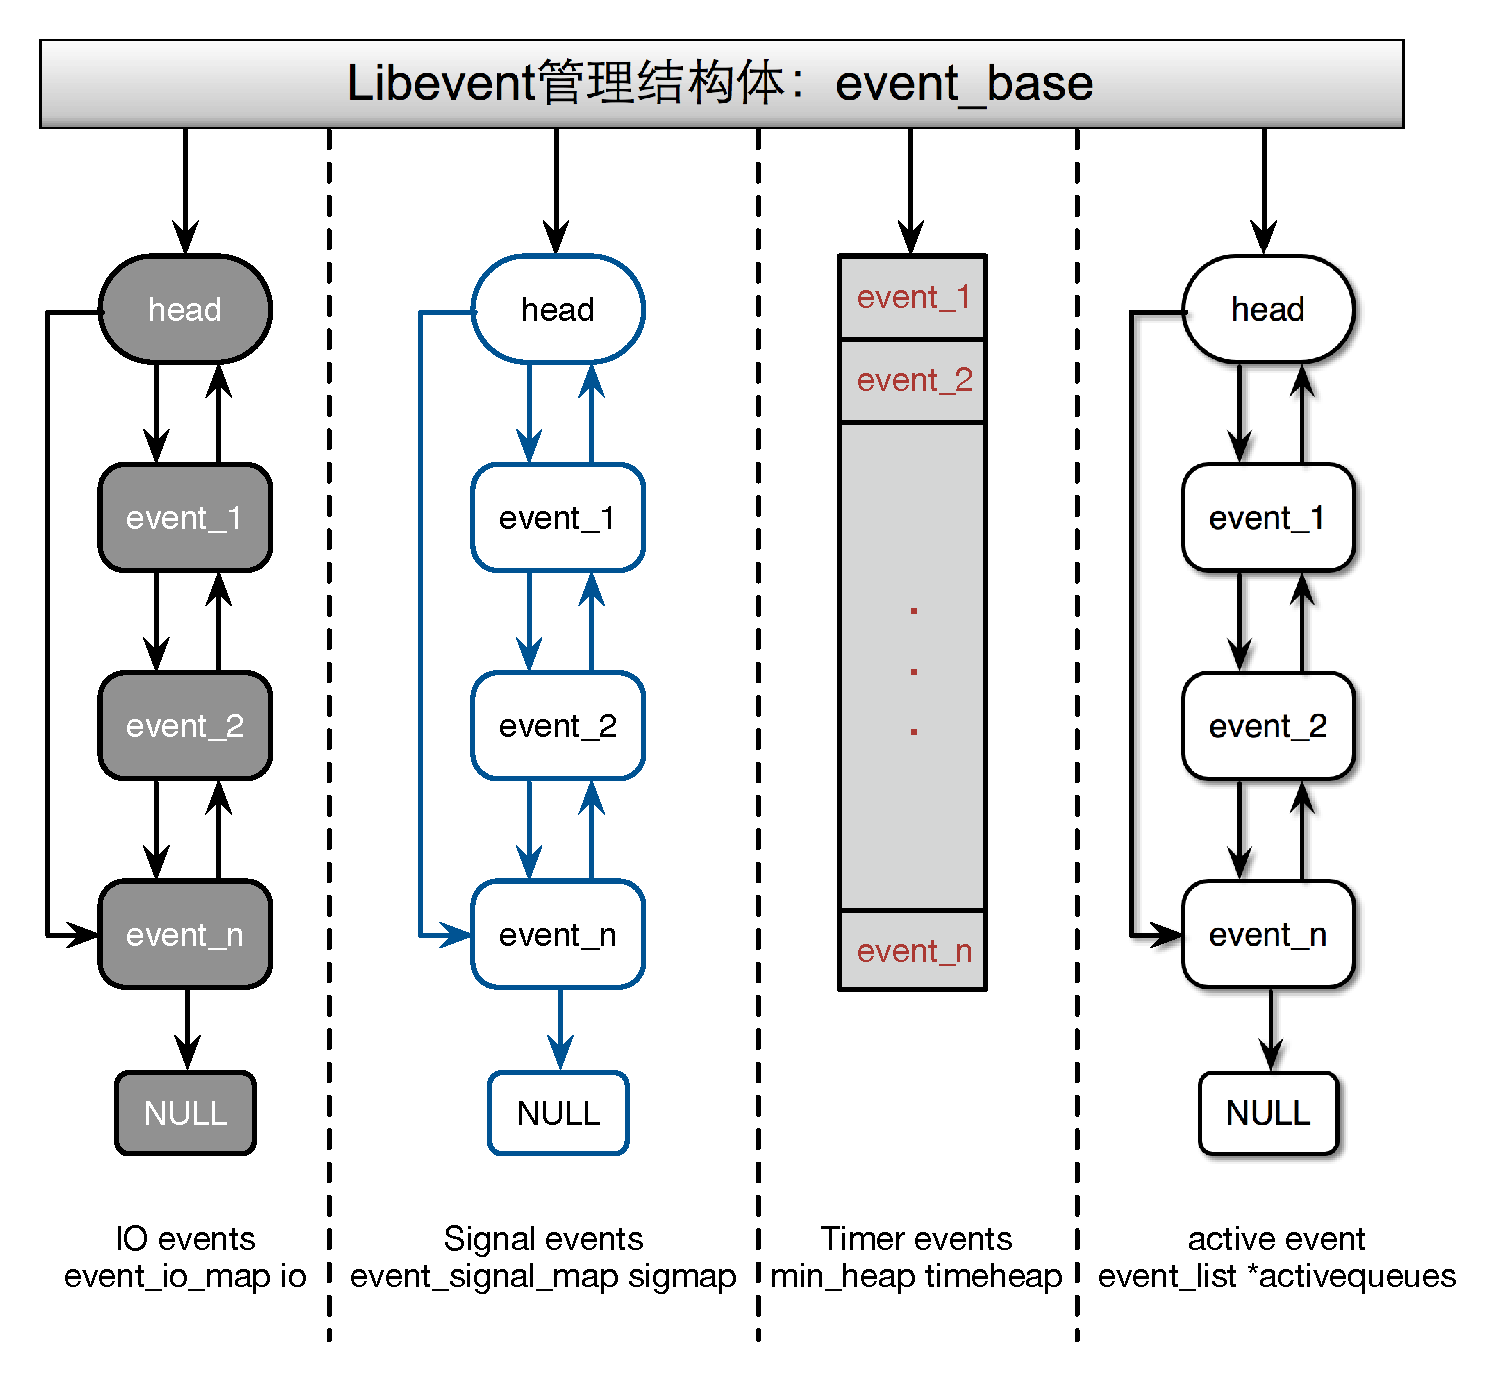
\includegraphics [width=0.75\textwidth]{EventsManagement}
\caption{Events Management.}
\end{center}
\end{figure}

\newpage

\section{多线程、锁、条件变量}\label{S.ThreadLock}

Libevent原生是没有多线程模型的,需要开发者自己编写多线程相关的代码。
有了多线程之后,会涉及到加锁、解锁、条件变量以及线程安全等相关内容。
evthread、lock相关的宏、函数、线程安全相关知识

\newpage

\section{Libevent之Reactor}\label{S.Reactor}
本章主要是Libevent对多路IO复用机制的封装。

\subsection{Reactor Vs Proactor}
一般情况下,I/O 复用机制需要事件分离器(event demultiplexor)。 事件分离器的作用:将那些读写事件源分发给各读写事件的处理者。开发人员在开始的时候需要在分离器那里注册需要关注的事件,并提供相应的处理者(event handlers),或者是回调函数; 事件分离器在适当的时候会将请求的事件分发给这些handler或者回调函数。

目前,事件分用器存在两种模式:Reactor和Proactor。 Reactor模式基于同步I/O,而Proactor模式基于异步I/O。 在Reactor模式中,事件分离器等待某个事件的发生(比如文件描述符可读写、socket可读写、定时器超时或者信号),事件分离器将此事件传给事先注册的事件处理函数或回调函数,由后者来做实际的读写操作。

而在Proactor模式中,事件处理者(或由事件分离器发起)直接发起一个异步读写操作(相当于请求),而实际工作是由操作系统完成的。发起时,需要提供的参数包括存放读到数据的缓冲区,读的数据大小,或者存放外发数据的缓冲区,以及这个请求完后的回调函数等信息。事件分离器得知了这个请求,它默默等待这个请求的完成,然后转发{\heiti 完成事件}给相应的事件处理者或者回调。

为了更好地理解Reactor与Proactor两种模式的区别,下面用read操作的例子来看一下两者的步骤。
下面是Reactor的做法:
\begin{enumerate}
\item 某事件处理者向事件分离器注册某个socket上的读事件;
\item 事件分离者等着这个事件的发生(可能会有一些其他事件);
\item 当事件发生了,事件分离器被唤醒,将读事件分发给相应事件处理者;
\item 事件处理者于是去那个socket上读数据。 若需要,它再次注册socket上的读事件,重复上面的步骤。
\end{enumerate}

下面再来看看Proactor(需要操作系统支持)是如何做的:
\begin{enumerate}
\item 事件处理者直接请求一个读操作,然后等待该读操作的完成;
\item 事件分离器等着这个读事件的完成,等待该事件的完成事件;
\item 事件分离器等待的同时,OS已经在执行该读操作:读取目标数据,放入用户提供的缓冲区中,最后通知事件分离器,即完成事件;
\item 事件分离器通知之前的事件处理者: 该读事件已经完成;
\item 事件处理者即可处理该读操作获得的数据。若需要,事件处理者再次请求一个写操作,重复上述几个步骤。
\end{enumerate}

按照大多数人的观点,Proactor的性能会比Reactor好(暂时没有实验测试)。目前windows、linux都有对异步IO的支持。也有一些网络库已经支持Proactor模式。Libevent采用的是Reactor模式,其实现了跨平台的多路IO复用接口封装。这使得用户可以在不同的平台使用统一的接口。接下来就讲一讲其跨平台的实现。
\footnote{由于Libevent库是一个通用的开源网络库,考虑到应用环境的多样性,故其实现了多路IO复用的封装。但在许多实际应用场景中,跨平台是没有必要的。}

\subsection{Reactor相关结构体}
下面代码是Libevent实现跨平台IO多路复用的相关数据结构:
\begin{lstlisting}[language=C]
`//event-internal.h文件`
struct event_base {  
	const struct eventop *evsel;	`//多路IO复用函数指针结构体`
	void *evbase;				  `//`
	……	
};

struct eventop {
	const char *name;				`//多路IO复用函数的名字`

	void *(*init)(struct event_base *);
	int (*add)(struct event_base *, evutil_socket_t fd, short old, short events, void *fdinfo);
	int (*del)(struct event_base *, evutil_socket_t fd, short old, short events, void *fdinfo);
	int (*dispatch)(struct event_base *, struct timeval *);
	void (*dealloc)(struct event_base *);

	int need_reinit;  					`//是否要重新初始化,0表示不需要`
	enum event_method_feature features;      `//多路IO复用的特征,详见下文解释`
	size_t fdinfo_len;					`//额外信息的长度。有些多路IO复用函数需要额外的信息`
};
\end{lstlisting}
event\_base结构体是Libevent中最核心的结构体,其详细介绍参见第\ref{S.MainStructure}章。此处我们关注evsel和evbase成员。evsel是一个struct eventop结构体指针,struct eventop的成员是一些函数指针,实际上这些函数指针最终指向的就是多路IO复用函数中对应的函数。只需要给这些指针赋予相应的多路IO复用的函数即可。
\begin{itemize}
\item init {Function to set up an event\_base to use this backend.  It should create a new structure holding whatever information is needed to run the backend, and return it.  The returned pointer will get stored by event\_init into the event\_base.evbase field.  On failure, this function should return NULL. }
\item add {Enable reading/writing on a given fd or signal.  'events' will be the events that we're trying to enable: one or more of EV\_READ, EV\_WRITE, EV\_SIGNAL, and EV\_ET.  'old' will be those events that were enabled on this fd previously.  'fdinfo' will be a structure associated with the fd by the evmap; its size is defined by the fdinfo field below.  It will be set to 0 the first time the fd is added.  The function should return 0 on success and -1 on error.}
\item del { As "add", except 'events' contains the events we mean to disable.}
\item dispatch可以进入监听 {Function to implement the core of an event loop.  It must see which added events are ready, and cause event\_active to be called for each active event (usually via event\_io\_active or such).  It should return 0 on success and -1 on error.}。
\item dealloc {Function to clean up and free our data from the event\_base.}
\end{itemize}

feature成员指定多路IO复用函数应该满足哪些特征。所有的特征定义在一个枚举类型中,在使用中可以调用event\_config\_avoid\_method()可以通过名字让libevent避免使用特定的可用后端。调用event\_config\_require\_feature()让libevent不使用不能提供所有指定特征的后端,event\_config\_require\_features()可识别的特征值有:
\begin{lstlisting}[language=C]
`//event.h文件`
enum event_method_feature {
	EV_FEATURE_ET = 0x01,       `//支持边沿触发`
	EV_FEATURE_O1 = 0x02,       `//要求事件分派器时间复杂度为O(1),排除select、poll等`
	EV_FEATURE_FDS = 0x04      `//支持任意文件描述符,而不能仅仅支持套接字`
};
\end{lstlisting}

\subsection{多路IO复用机制}
现有的许多平台都有不止一种多路IO复用机制,例如Linux就支持select、poll、epoll,而BSD支持的包括select、kqueue。关于各个多路IO复用机制此处没有详细介绍,网络上有许多很好的资料。Libevent支持的多路IO复用机制包括:select、poll、epoll、kqueue、devpoll等。其封装都在相对应的代码文件里,例如select的函数接口声明如下:
\begin{lstlisting}[language=C]
`//select.c文件`
static void *select_init(struct event_base *);
static int select_add(struct event_base *, int, short old, short events, void*);
static int select_del(struct event_base *, int, short old, short events, void*);
static int select_dispatch(struct event_base *, struct timeval *);
static void select_dealloc(struct event_base *);

const struct eventop selectops = {
	"select",
	select_init,
	select_add,
	select_del,
	select_dispatch,
	select_dealloc,
	0, EV_FEATURE_FDS, 0,
};  
\end{lstlisting}

有些多路IO复用机制的实现相比这个两个会复杂一些,如epoll、kqueue等。
\begin{lstlisting}[language=C]
`//epoll.c文件`
static void *epoll_init(struct event_base *);
static int epoll_dispatch(struct event_base *, struct timeval *);
static void epoll_dealloc(struct event_base *);

static const struct eventop epollops_changelist = {
	"epoll (with changelist)",
	epoll_init,
	event_changelist_add,
	event_changelist_del,
	epoll_dispatch,
	epoll_dealloc,
	1,
	EV_FEATURE_ET|EV_FEATURE_O1,
	EVENT_CHANGELIST_FDINFO_SIZE
};

static int epoll_nochangelist_add(struct event_base *base, evutil_socket_t fd,
    short old, short events, void *p);
static int epoll_nochangelist_del(struct event_base *base, evutil_socket_t fd,
    short old, short events, void *p);

const struct eventop epollops = {
	"epoll",
	epoll_init,
	epoll_nochangelist_add,
	epoll_nochangelist_del,
	epoll_dispatch,
	epoll_dealloc,
	1,
	EV_FEATURE_ET|EV_FEATURE_O1,
	0
};
\end{lstlisting}

注意到epoll定义了两个struct eventop结构,直观的观察,是前者是使用的基于changelist的事件添加删除函数,而后者使用epoll自带的相关函数接口。这个可以调用event\_config\_set\_flag()让libevent在创建event\_base时设置一个或者多个将在下面介绍的运行时标志,event\_config\_set\_flag()可识别的选项值有:
\begin{lstlisting}[language=C]
enum event_base_config_flag {
	EVENT_BASE_FLAG_NOLOCK = 0x01,
	EVENT_BASE_FLAG_IGNORE_ENV = 0x02,
	EVENT_BASE_FLAG_STARTUP_IOCP = 0x04,
	EVENT_BASE_FLAG_NO_CACHE_TIME = 0x08,
	EVENT_BASE_FLAG_EPOLL_USE_CHANGELIST = 0x10
};
\end{lstlisting}
\begin{itemize}
\item EVENT\_BASE\_FLAG\_NOLOCK:不要为event\_base分配锁。设置这个选项可以为event\_base节省一点用于锁定和解锁的时间,但是让在多个线程中访问event\_base成为不安全的。
\item EVENT\_BASE\_FLAG\_IGNORE\_ENV:选择使用的后端时,不要检测EVENT\_*环境变量。使用这个标志需要三思:这会让用户更难调试你的程序与libevent的交互。
\item EVENT\_BASE\_FLAG\_STARTUP\_IOCP:仅用于Windows,让libevent在启动时就启用任何必需的IOCP分发逻辑,而不是按需启用。
\item EVENT\_BASE\_FLAG\_NO\_CACHE\_TIME:不是在事件循环每次准备执行超时回调时检测当前时间,而是在每次超时回调后进行检测。注意:这会消耗更多的CPU时间。
\item EVENT\_BASE\_FLAG\_EPOLL\_USE\_CHANGELIST:告诉libevent,如果使用epoll后端,可以安全地使用更快的基于changelist的后端。epoll-changelist后端可以在后端的分发函数调用之间,同样的fd多次修改其状态的情况下,避免不必要的系统调用。但如果传递任何使用dup()或者其变体克隆的fd给libevent,epoll-changelist后端会触发一个内核bug,导致不正确的结果。在不使用epoll后端的情况下,这个标志无效。也可以通过设置EVENT\_EPOLL\_USE\_CHANGELIST环境变量来打开epoll-changelist选项。
\end{itemize}

【比较基于changelist和非changelist之间的区别】

\subsection{选择多路IO复用后端}
看到这里,想必已经知道,只需将对应平台的多路IO复用函数的全局变量赋值给event\_base的evsel变量即可。可是怎么让Libevent根据不同的平台选择不同的多路IO复用函数呢?另外大部分OS都会实现select、poll和一个自己的高效多路IO复用函数。怎么从多个中选择一个甚至是最优的呢?下面看一下Libevent的解决方案:
\begin{lstlisting}[language=C]
`//event.c文件`
#ifdef _EVENT_HAVE_EVENT_PORTS  
extern const struct eventop evportops;
#endif
#ifdef _EVENT_HAVE_SELECT
extern const struct eventop selectops;
#endif
#ifdef _EVENT_HAVE_POLL
extern const struct eventop pollops;
#endif
#ifdef _EVENT_HAVE_EPOLL
extern const struct eventop epollops;
#endif
#ifdef _EVENT_HAVE_WORKING_KQUEUE
extern const struct eventop kqops;
#endif
#ifdef _EVENT_HAVE_DEVPOLL
extern const struct eventop devpollops;
#endif
#ifdef WIN32
extern const struct eventop win32ops;
#endif

static const struct eventop *eventops[] = {
#ifdef _EVENT_HAVE_EVENT_PORTS
	&evportops,
#endif
#ifdef _EVENT_HAVE_WORKING_KQUEUE
	&kqops,
#endif
#ifdef _EVENT_HAVE_EPOLL
	&epollops,
#endif
#ifdef _EVENT_HAVE_DEVPOLL
	&devpollops,
#endif
#ifdef _EVENT_HAVE_POLL
	&pollops,
#endif
#ifdef _EVENT_HAVE_SELECT
	&selectops,
#endif
#ifdef WIN32
	&win32ops,
#endif
	NULL
};
\end{lstlisting}

它根据宏定义判断当前的OS环境是否有某个多路IO复用函数。如果有,那么就把与之对应的struct eventop结构体指针放到一个全局数组中。有了这个数组,现在只需将数组的某个元素赋值给evsel变量即可。因为是条件宏,在编译器编译代码之前完成宏的替换,所以是可以这样定义一个数组的。这些宏都在event-config.h中有定义了,该文件是一个很基础和重要的文件。在文件的一开始有这样一句"This file was generated by autoconf when libevent was built"。这说明这个文件是在Libevent配置的时候生成的,即在编译Libevent之前就应该要生成该文件。

从数组的元素可以看到,低下标存的是高效多路IO复用函数。如果从低到高下标选取一个多路IO复用函数,那么将优先选择高效的。现在看一下Libevent如何选取后端:
\begin{lstlisting}[language=C]
//event.c文件
struct event_base *event_base_new_with_config(const struct event_config *cfg) {  
	int i;
	struct event_base *base;
	int should_check_environment;

	`/* 分配并清零event\_base内存. event\_base所有成员均初始化为0 */`
	if ((base = mm_calloc(1, sizeof(struct event_base))) == NULL) {
		event_warn("%s: calloc", __func__);
		return NULL;
	}
	...……
	should_check_environment =
		!(cfg && (cfg->flags & EVENT_BASE_FLAG_IGNORE_ENV));
	`/* 遍历数组元素 */`
	for (i = 0; eventops[i] && !base->evbase; i++) {
		if (cfg != NULL) {
		`/* 判断该后端是否被禁用 */`
		if (event_config_is_avoided_method(cfg, eventops[i]->name))
			continue;
		if ((eventops[i]->features & cfg->require_features) != cfg->require_features)
			continue;
		}

		`/* also obey the environment variables */ `
		if (should_check_environment && event_is_method_disabled(eventops[i]->name))
			continue;
  
		`/* 找到一个满足条件的多路IO复用后端 */`
		base->evsel = eventops[i];

		base->evbase = base->evsel->init(base);
	}

	if (base->evbase == NULL) {
		event_warnx("%s: no event mechanism available",  __func__);
		base->evsel = NULL;
		event_base_free(base);
		return NULL;
	}
	……
	return (base);
} 
\end{lstlisting}
event\_base\_new\_with\_config用于根据event\_config来创建event\_base,将会在下一章详细介绍。此处关注其中的for循环,可以看到,首先从eventops数组中选出一个元素。如果设置了event\_config,那么就对这个元素(即多路IO复用函数)特征进行检测,看其是否满足event\_config所描述的特征。找到第一个符合条件的eventops元素并赋值给evsel,根据for循环的判断条件:eventops[i] \&\& !base->evbase,此for循环结束。

【此处添加对event\_config的解释】

后端数据存储结构体:
在本文最前面列出的event\_base结构体中,除了evsel变量外,还有一个evbase变量。这也是一个很重要的变量,而且也是用于跨平台的。像select、poll、epoll之类多路IO复用函数在调用时要传入一些数据,比如监听的文件描述符fd,监听了的哪些事件。在Libevent中,这些数据不是保存在event\_base这个结构体中的,而是存放在evbase这个指针指向的结构体中。

需要注意到evbase是void指针类型,这是由于不同的多路IO复用函数需要使用不同格式的数据,所以Libevent为每一个多路IO复用函数都定义了专门的结构体(即结构体是不同的),暂且称之为IO复用结构体。evbase指向的就是这些结构体。由于这些结构体是不同的,所以要用一个void类型指针。epoll的IO复用结构体,如下面代码所示:
\begin{lstlisting}[language=C]
`/* epoll.c文件 */`
struct epollop {
	struct epoll_event *events;
	int nevents;
	int epfd;
};
\end{lstlisting}

前面event\_base\_new\_with\_config的代码中,即该函数第34行,调用了init函数。这行代码就是用来赋值evbase的。下面是epoll对应的init函数:
\begin{lstlisting}[language=C]
`/* epoll.c文件 */`
static void *epoll_init(struct event_base *base) {
	int epfd;
	struct epollop *epollop;

	/* Initialize the kernel queue.  (The size field is ignored since 2.6.8.) */
	if ((epfd = epoll_create(32000)) == -1) {
		if (errno != ENOSYS)
			event_warn("epoll_create");
		return (NULL);
	}

	evutil_make_socket_closeonexec(epfd);

	if (!(epollop = mm_calloc(1, sizeof(struct epollop)))) {
		close(epfd);
		return (NULL);
	}

	epollop->epfd = epfd;

	/* Initialize fields */
	epollop->events = mm_calloc(INITIAL_NEVENT, sizeof(struct epoll_event));
	if (epollop->events == NULL) {
		mm_free(epollop);
		close(epfd);
		return (NULL);
	}
	epollop->nevents = INITIAL_NEVENT;

	if ((base->flags & EVENT_BASE_FLAG_EPOLL_USE_CHANGELIST) != 0 ||
	    ((base->flags & EVENT_BASE_FLAG_IGNORE_ENV) == 0 &&
		evutil_getenv("EVENT_EPOLL_USE_CHANGELIST") != NULL))
		base->evsel = &epollops_changelist;

	evsig_init(base);

	return (epollop);
}
\end{lstlisting}
经过上面的处理后,Libevent在特定的OS下能使用到特定的多路IO复用函数。在之前说到的evmap\_io\_add和evmap\_signal\_add函数中都会调用evsel->add。由于在新建event\_base时就选定了对应的多路IO复用函数,给evsel、evbase变量赋值,所以evsel->add能把对应的fd和监听事件加到对应的IO复用结构体保存。
由于有evsel和evbase这个两个指针变量,当初始化完成之后,再也不用担心具体使用的是哪个多路IO复用后端。evsel结构体的函数指针提供了统一的接口,上层的代码要使用到多路IO复用函数的一些操作函数时,直接调用evsel结构体提供的函数指针即可。也正是如此,Libevent实现了统一的跨平台Reactor接口。

\newpage

\section{Libevent核心流程}
本章主要介绍Libevent的核心事件流程。event.c中的核心框架

\subsection{简单示例}
为了能够清晰的把握核心流程而不被细枝末节而打乱,首先看一个最简单的libevent的示例:
\begin{lstlisting}[language=C]
#include<unistd.h>
#include<stdio.h>
#include<thread.h>

#include<event2/event.h>

void example_cb(int fd, short events, void *arg) {
	char buf[512];
	printf("In the example_cb\n");
	read(fd, buf, sizeof(buf));
}

int main() {
	`/* 使用event\_base默认配置 */`
	struct event_base *base = event_base_new();

	struct event *example_ev = event_new(base, STDIN_FILENO,
                       EV_READ | EV_PERSIST, example_cb, NULL);

	event_add(example_ev, NULL); `/* 没有超时 */`

	event_base_dispatch(base);

	return 0;
}
\end{lstlisting}
这个例子已经包含了Libevent的基础工作流程。用event\_base\_new初始化一个event\_base结构体,这个结构体是libevent中核心数据结构,他将原本独立的各个单元整合在一起。然后event\_new创建一个event事件,该事件监听标准输入的读事件,并设置为永久事件(EV\_PERSIST)。再将此新创建的一个事件添加到event\_base中。最后调用事件分派函数,开始一直监听已经添加到event\_base中的事件。本章后面的内容将按照这样的主线进行分析。

\subsection{创建event\_base}
event\_base\_new函数可以创建一个默认配置的event\_base结构体。它先用event\_config\_new创建一个event\_config,这个配置结构体默认是空的,也就是说不包含任何配置信息,然后调用event\_base\_new\_with\_config函数创建默认配置的event\_base结构体。下面先看一下event\_base\_new\_with\_config:
\begin{lstlisting}[language=C]
`/* event.c文件 */`
struct event_base * event_base_new(void) {
	struct event_base *base = NULL;
	struct event_config *cfg = event_config_new();
	if (cfg) {
		base = event_base_new_with_config(cfg);
		event_config_free(cfg);
	}
	return base;
}

struct event_base * event_base_new_with_config(const struct event_config *cfg) {
	int i;
	struct event_base *base;
	int should_check_environment;

#ifndef _EVENT_DISABLE_DEBUG_MODE
	event_debug_mode_too_late = 1;
#endif

	if ((base = mm_calloc(1, sizeof(struct event_base))) == NULL) {
		event_warn("%s: calloc", __func__);
		return NULL;
	}
	detect_monotonic();
	gettime(base, &base->event_tv);

	min_heap_ctor(&base->timeheap);
	TAILQ_INIT(&base->eventqueue);
	base->sig.ev_signal_pair[0] = -1;
	base->sig.ev_signal_pair[1] = -1;
	base->th_notify_fd[0] = -1;
	base->th_notify_fd[1] = -1;

	event_deferred_cb_queue_init(&base->defer_queue);
	base->defer_queue.notify_fn = notify_base_cbq_callback;
	base->defer_queue.notify_arg = base;
	if (cfg)
		base->flags = cfg->flags;

	evmap_io_initmap(&base->io);
	evmap_signal_initmap(&base->sigmap);
	event_changelist_init(&base->changelist);

	base->evbase = NULL;

	should_check_environment =
	    !(cfg && (cfg->flags & EVENT_BASE_FLAG_IGNORE_ENV));

	`/* 选择IO复用后端,前文已经讲解过 */`
	……

	if (base->evbase == NULL) {
		event_warnx("%s: no event mechanism available", __func__);
		base->evsel = NULL;
		event_base_free(base);
		return NULL;
	}

	if (evutil_getenv("EVENT_SHOW_METHOD"))
		event_msgx("libevent using: %s", base->evsel->name);

	/* allocate a single active event queue */
	if (event_base_priority_init(base, 1) < 0) {
		event_base_free(base);
		return NULL;
	}

	/* prepare for threading */
#ifndef _EVENT_DISABLE_THREAD_SUPPORT
	`//测试evthread\_lock\_callbacks结构中的lock指针函数是否为NULL
	//即测试Libevent是否已经初始化为支持多线程模式。
	//由于一开始是用mm\_calloc申请内存的,所以该内存区域的值为0
	//对于th\_base\_lock变量,目前的值为NULL.`
	if (EVTHREAD_LOCKING_ENABLED() &&
	    (!cfg || !(cfg->flags & EVENT_BASE_FLAG_NOLOCK))) {
		int r;
		EVTHREAD_ALLOC_LOCK(base->th_base_lock,
		    EVTHREAD_LOCKTYPE_RECURSIVE);
		base->defer_queue.lock = base->th_base_lock;
		EVTHREAD_ALLOC_COND(base->current_event_cond);
		r = evthread_make_base_notifiable(base);
		if (r<0) {
			event_warnx("%s: Unable to make base notifiable.", __func__);
			event_base_free(base);
			return NULL;
		}
	}
#endif

#ifdef WIN32
	……
#endif

	return (base);
}
\end{lstlisting}
有时,需要对某些方面有些特殊的要求,此时就不能使用默认配置的event\_base了,需要对event\_base进行配置。这里用到了event\_config结构体,【配置event\_base】。这个结构体主要是对event\_base进行一些配置。

宏EVTHREAD\_LOCKING\_ENABLED主要是检测是否已经支持锁了。检测的方式也很简单,也就是检测\_evthread\_lock\_fns全局变量中的lock成员变量是否不为NULL。有关这个\_evthread\_lock\_fns全局变量在【多线程、锁、条件变量】中讲解。

\subsection{创建event}
现在event\_base已经新建出来了。下面看一下event\_new函数,它和前面的event\_base\_new一样,把主要是的初始化工作交给另一个函数。event\_new函数的工作只是创建一个struct event结构体,然后把它的参数原封不动地传给event\_assign,所以还是看event\_assign函数。

\begin{lstlisting}[language=C]
struct event *event_new(struct event_base *base, evutil_socket_t fd, short events, 
					void (*cb)(evutil_socket_t, short, void *), void *arg) {
	struct event *ev;
	ev = mm_malloc(sizeof(struct event));
	if (ev == NULL)
		return (NULL);
	if (event_assign(ev, base, fd, events, cb, arg) < 0) {
		mm_free(ev);
		return (NULL);
	}

	return (ev);
}

int event_assign(struct event *ev, struct event_base *base, evutil_socket_t fd,
			  short events, void (*callback)(evutil_socket_t, short, void *), void *arg) {
	if (!base)
		base = current_base;

	_event_debug_assert_not_added(ev);

	ev->ev_base = base;

	ev->ev_callback = callback;
	ev->ev_arg = arg;
	ev->ev_fd = fd;
	ev->ev_events = events;
	ev->ev_res = 0;
	ev->ev_flags = EVLIST_INIT;
	ev->ev_ncalls = 0;
	ev->ev_pncalls = NULL;

	if (events & EV_SIGNAL) {
		if ((events & (EV_READ|EV_WRITE)) != 0) {
			event_warnx("%s: EV_SIGNAL is not compatible with "
			    "EV_READ or EV_WRITE", __func__);
			return -1;
		}
		ev->ev_closure = EV_CLOSURE_SIGNAL;
	} else {
		if (events & EV_PERSIST) {
			evutil_timerclear(&ev->ev_io_timeout);
			ev->ev_closure = EV_CLOSURE_PERSIST;
		} else {
			ev->ev_closure = EV_CLOSURE_NONE;
		}
	}

	min_heap_elem_init(ev);

	if (base != NULL) {
		/* by default, we put new events into the middle priority */
		ev->ev_pri = base->nactivequeues / 2;
	}

	_event_debug_note_setup(ev);

	return 0;
}
\end{lstlisting}

从event\_assign函数的名字可以得知它是进行赋值操作的。所以它能可以在event被初始化后再次调用。不过,初始化后再次调用的话,有些事情要注意。【注意事项】
从上面的代码可看到:如果这个event是用来监听一个信号的,那么就不能让这个event监听读或者写事件。
注意,此时event结构体的变量ev\_flags的值是EVLIST\_INIT。对变量的追踪是很有帮助的。它指明了event结构体的状态。它通过以或运算的方式取下面的值:

\begin{lstlisting}[language=C] 
//event_struct.h文件
#define EVLIST_TIMEOUT	0x01		//event从属于定时器队列或者时间堆
#define EVLIST_INSERTED	0x02		//event从属于注册队列
#define EVLIST_SIGNAL	0x04			//没有使用
#define EVLIST_ACTIVE	0x08			//event从属于活动队列
#define EVLIST_INTERNAL	0x10		//该event是内部使用的。信号处理时有用到
#define EVLIST_INIT	0x80			//event已经被初始化了

/* EVLIST_X_ Private space: 0x1000-0xf000 */
#define EVLIST_ALL	(0xf000 | 0x9f)		//所有标志。这个不能取
\end{lstlisting}

\subsection{向event\_base添加event}
创建完一个event结构体后,现在看一下event\_add。它同前面的函数一样,内部也是调用其他函数完成工作。因为它用到了锁,所以给出它的代码。
\begin{lstlisting}[language=C]
int event_add(struct event *ev, const struct timeval *tv) {
	int res;

	if (EVUTIL_FAILURE_CHECK(!ev->ev_base)) {
		event_warnx("%s: event has no event_base set.", __func__);
		return -1;
	}

	EVBASE_ACQUIRE_LOCK(ev->ev_base, th_base_lock);

	res = event_add_internal(ev, tv, 0);

	EVBASE_RELEASE_LOCK(ev->ev_base, th_base_lock);

	return (res);
}

/* Implementation function to add an event.  Works just like event_add,
 * except: 1) it requires that we have the lock.  2) if tv_is_absolute is set,
 * we treat tv as an absolute time, not as an interval to add to the current
 * time */
static inline int event_add_internal(struct event *ev, const struct timeval *tv, int tv_is_absolute) {
	struct event_base *base = ev->ev_base;
	int res = 0;
	int notify = 0;

	EVENT_BASE_ASSERT_LOCKED(base);
	_event_debug_assert_is_setup(ev);

	event_debug((
		 "event_add: event: %p (fd "EV_SOCK_FMT"), %s%s%scall %p",
		 ev,
		 EV_SOCK_ARG(ev->ev_fd),
		 ev->ev_events & EV_READ ? "EV_READ " : " ",
		 ev->ev_events & EV_WRITE ? "EV_WRITE " : " ",
		 tv ? "EV_TIMEOUT " : " ",
		 ev->ev_callback));

	EVUTIL_ASSERT(!(ev->ev_flags & ~EVLIST_ALL));

	/*
	 * prepare for timeout insertion further below, if we get a
	 * failure on any step, we should not change any state.
	 */
	if (tv != NULL && !(ev->ev_flags & EVLIST_TIMEOUT)) {
		if (min_heap_reserve(&base->timeheap,
			1 + min_heap_size(&base->timeheap)) == -1)
			return (-1);  /* ENOMEM == errno */
	}

	/* If the main thread is currently executing a signal event's
	 * callback, and we are not the main thread, then we want to wait
	 * until the callback is done before we mess with the event, or else
	 * we can race on ev_ncalls and ev_pncalls below. */
#ifndef _EVENT_DISABLE_THREAD_SUPPORT
	if (base->current_event == ev && (ev->ev_events & EV_SIGNAL)
	    && !EVBASE_IN_THREAD(base)) {
		++base->current_event_waiters;
		EVTHREAD_COND_WAIT(base->current_event_cond, base->th_base_lock);
	}
#endif

	if ((ev->ev_events & (EV_READ|EV_WRITE|EV_SIGNAL)) &&
	    !(ev->ev_flags & (EVLIST_INSERTED|EVLIST_ACTIVE))) {
		if (ev->ev_events & (EV_READ|EV_WRITE))
			res = evmap_io_add(base, ev->ev_fd, ev);
		else if (ev->ev_events & EV_SIGNAL)
			res = evmap_signal_add(base, (int)ev->ev_fd, ev);
		if (res != -1)
			event_queue_insert(base, ev, EVLIST_INSERTED);
		if (res == 1) {
			/* evmap says we need to notify the main thread. */
			notify = 1;
			res = 0;
		}
	}

	/*
	 * we should change the timeout state only if the previous event
	 * addition succeeded.
	 */
	if (res != -1 && tv != NULL) {
		struct timeval now;
		int common_timeout;

		/*
		 * for persistent timeout events, we remember the
		 * timeout value and re-add the event.
		 *
		 * If tv_is_absolute, this was already set.
		 */
		if (ev->ev_closure == EV_CLOSURE_PERSIST && !tv_is_absolute)
			ev->ev_io_timeout = *tv;

		/*
		 * we already reserved memory above for the case where we
		 * are not replacing an existing timeout.
		 */
		if (ev->ev_flags & EVLIST_TIMEOUT) {
			/* XXX I believe this is needless. */
			if (min_heap_elt_is_top(ev))
				notify = 1;
			event_queue_remove(base, ev, EVLIST_TIMEOUT);
		}

		/* Check if it is active due to a timeout.  Rescheduling
		 * this timeout before the callback can be executed
		 * removes it from the active list. */
		if ((ev->ev_flags & EVLIST_ACTIVE) &&
		    (ev->ev_res & EV_TIMEOUT)) {
			if (ev->ev_events & EV_SIGNAL) {
				/* See if we are just active executing
				 * this event in a loop
				 */
				if (ev->ev_ncalls && ev->ev_pncalls) {
					/* Abort loop */
					*ev->ev_pncalls = 0;
				}
			}

			event_queue_remove(base, ev, EVLIST_ACTIVE);
		}

		gettime(base, &now);

		common_timeout = is_common_timeout(tv, base);
		if (tv_is_absolute) {
			ev->ev_timeout = *tv;
		} else if (common_timeout) {
			struct timeval tmp = *tv;
			tmp.tv_usec &= MICROSECONDS_MASK;
			evutil_timeradd(&now, &tmp, &ev->ev_timeout);
			ev->ev_timeout.tv_usec |=
			    (tv->tv_usec & ~MICROSECONDS_MASK);
		} else {
			evutil_timeradd(&now, tv, &ev->ev_timeout);
		}

		event_debug((
			 "event_add: timeout in %d seconds, call %p",
			 (int)tv->tv_sec, ev->ev_callback));

		event_queue_insert(base, ev, EVLIST_TIMEOUT);
		if (common_timeout) {
			struct common_timeout_list *ctl =
			    get_common_timeout_list(base, &ev->ev_timeout);
			if (ev == TAILQ_FIRST(&ctl->events)) {
				common_timeout_schedule(ctl, &now, ev);
			}
		} else {
			/* See if the earliest timeout is now earlier than it
			 * was before: if so, we will need to tell the main
			 * thread to wake up earlier than it would
			 * otherwise. */
			if (min_heap_elt_is_top(ev))
				notify = 1;
		}
	}

	/* if we are not in the right thread, we need to wake up the loop */
	if (res != -1 && notify && EVBASE_NEED_NOTIFY(base))
		evthread_notify_base(base);

	_event_debug_note_add(ev);

	return (res);
}
\end{lstlisting}
event\_add函数只是对event\_base加了锁,然后调用event\_add\_internal函数完成工作。所以函数event\_add是线程安全的。
event\_add\_internal函数会调用evmap\_io\_add和evmap\_signal\_add,把有相同文件描述符fd和信号值sig的event连在一个队列里面。成功之后,就会调用event\_queue\_insert,向event\_base注册事件。

【evmap\_io\_add和evmap\_signal\_add函数】把要监听的fd或者sig添加到多路IO复用函数中,使得其是可以监听的。

\begin{lstlisting}[language=C]
//evmap.c文件
int evmap_io_add(struct event_base *base, evutil_socket_t fd, struct event *ev) {
	const struct eventop *evsel = base->evsel;
	struct event_io_map *io = &base->io;
	struct evmap_io *ctx = NULL;
	int nread, nwrite, retval = 0;
	short res = 0, old = 0;
	struct event *old_ev;

	……

	//GET_IO_SLOT_AND_CTOR宏的作用就是让ctx指向struct event_map_entry结构体中的TAILQ_HEAD
	//宏的展开,可以到http://blog.csdn.net/luotuo44/article/details/38403241查看
	GET_IO_SLOT_AND_CTOR(ctx, io, fd, evmap_io, evmap_io_init,
						 evsel->fdinfo_len);

    //同一个fd可以调用event_new,event_add
    //多次。nread、nwrite就是记录有多少次。如果每次event_new的回调函数
    //都不一样,那么当fd有可读或者可写时,这些回调函数都是会触发的。
    //对一个fd不能event_new、event_add太多次的。后面会进行判断
    nread = ctx->nread;
    nwrite = ctx->nwrite;

    if (nread)
        old |= EV_READ;
    if (nwrite)
        old |= EV_WRITE;

    if (ev->ev_events & EV_READ) {
        //记录是不是第一次。如果是第一次,那么就说明该fd还没被
        //加入到多路IO复用中。即还没被加入到像select、epoll这些
        //函数中。那么就要加入。这个在后面可以看到。
        if (++nread == 1)
            res |= EV_READ;
    }
    if (ev->ev_events & EV_WRITE) {
        if (++nwrite == 1)
            res |= EV_WRITE;
    }
    if (EVUTIL_UNLIKELY(nread > 0xffff || nwrite > 0xffff)) {
        event_warnx("Too many events reading or writing on fd %d",
                    (int)fd);
        return -1;
    }

    //把fd加入到多路IO复用中。
    if (res) {
        void *extra = ((char*)ctx) + sizeof(struct evmap_io);
        if (evsel->add(base, ev->ev_fd,
                       old, (ev->ev_events & EV_ET) | res, extra) == -1)
            return (-1);
        retval = 1;
    }

    //nread进行了++。把次数记录下来。下次对于同一个fd,这个次数就有用了
    ctx->nread = (ev_uint16_t) nread;
    ctx->nwrite = (ev_uint16_t) nwrite;

    TAILQ_INSERT_TAIL(&ctx->events, ev, ev_io_next);

    return (retval);
}
\end{lstlisting}
代码中有两个计数nread和nwrite,当其值为1时,就说明是第一次监听对应的事件。此时,就要把这个fd添加到多路IO复用函数中。这就完成fd与select、poll、epoll之类的多路IO复用函数的相关联。这完成对fd监听的第一步。

\begin{lstlisting}[language=C]
//
static void event_queue_insert(struct event_base *base, struct event *ev, int queue)
{
	EVENT_BASE_ASSERT_LOCKED(base);

	if (ev->ev_flags & queue) {
		/* Double insertion is possible for active events */
		if (queue & EVLIST_ACTIVE)
			return;

		event_errx(1, "%s: %p(fd "EV_SOCK_FMT") already on queue %x", __func__,
		    ev, EV_SOCK_ARG(ev->ev_fd), queue);
		return;
	}

	if (~ev->ev_flags & EVLIST_INTERNAL)
		base->event_count++;

	ev->ev_flags |= queue;
	switch (queue) {
	case EVLIST_INSERTED:
		TAILQ_INSERT_TAIL(&base->eventqueue, ev, ev_next);
		break;
	case EVLIST_ACTIVE:
		base->event_count_active++;
		TAILQ_INSERT_TAIL(&base->activequeues[ev->ev_pri],
		    ev,ev_active_next);
		break;
	case EVLIST_TIMEOUT: {
		if (is_common_timeout(&ev->ev_timeout, base)) {
			struct common_timeout_list *ctl =
			    get_common_timeout_list(base, &ev->ev_timeout);
			insert_common_timeout_inorder(ctl, ev);
		} else
			min_heap_push(&base->timeheap, ev);
		break;
	}
	default:
		event_errx(1, "%s: unknown queue %x", __func__, queue);
	}
}
\end{lstlisting}
这个函数的主要作为是把event加入到对应的队列中。在这里,是为了把event加入到eventqueue这个已注册队列中,即将event向event\_base注册。注意,此时event结构体的ev\_flags变量为EVLIST\_INIT | EVLIST\_INSERTED了。

\subsection{监听event}       
现在事件已经添加完毕,开始进入主循环event\_base\_dispatch函数。还是同样,该函数内部调用event\_base\_loop完成工作。
\begin{lstlisting}[language=C]
int event_base_dispatch(struct event_base *event_base) {
	return (event_base_loop(event_base, 0));
}

int event_base_loop(struct event_base *base, int flags) {
	const struct eventop *evsel = base->evsel;
	struct timeval tv;
	struct timeval *tv_p;
	int res, done, retval = 0;

	/* Grab the lock.  We will release it inside evsel.dispatch, and again
	 * as we invoke user callbacks. */
	EVBASE_ACQUIRE_LOCK(base, th_base_lock);

	if (base->running_loop) {
		event_warnx("%s: reentrant invocation.  Only one event_base_loop"
		    " can run on each event_base at once.", __func__);
		EVBASE_RELEASE_LOCK(base, th_base_lock);
		return -1;
	}

	base->running_loop = 1;

	clear_time_cache(base);

	if (base->sig.ev_signal_added && base->sig.ev_n_signals_added)
		evsig_set_base(base);

	done = 0;

#ifndef _EVENT_DISABLE_THREAD_SUPPORT
	base->th_owner_id = EVTHREAD_GET_ID();
#endif

	base->event_gotterm = base->event_break = 0;

	while (!done) {
		base->event_continue = 0;

		/* Terminate the loop if we have been asked to */
		if (base->event_gotterm) {
			break;
		}

		if (base->event_break) {
			break;
		}

		timeout_correct(base, &tv);

		tv_p = &tv;
		if (!N_ACTIVE_CALLBACKS(base) && !(flags & EVLOOP_NONBLOCK)) {
			timeout_next(base, &tv_p);
		} else {
			/*
			 * if we have active events, we just poll new events
			 * without waiting.
			 */
			evutil_timerclear(&tv);
		}

		/* If we have no events, we just exit */
		if (!event_haveevents(base) && !N_ACTIVE_CALLBACKS(base)) {
			event_debug(("%s: no events registered.", __func__));
			retval = 1;
			goto done;
		}

		/* update last old time */
		gettime(base, &base->event_tv);

		clear_time_cache(base);

		res = evsel->dispatch(base, tv_p);

		if (res == -1) {
			event_debug(("%s: dispatch returned unsuccessfully.",
				__func__));
			retval = -1;
			goto done;
		}

		update_time_cache(base);

		timeout_process(base);

		if (N_ACTIVE_CALLBACKS(base)) {
			int n = event_process_active(base);
			if ((flags & EVLOOP_ONCE)
			    && N_ACTIVE_CALLBACKS(base) == 0
			    && n != 0)
				done = 1;
		} else if (flags & EVLOOP_NONBLOCK)
			done = 1;
	}
	event_debug(("%s: asked to terminate loop.", __func__));

done:
	clear_time_cache(base);
	base->running_loop = 0;

	EVBASE_RELEASE_LOCK(base, th_base_lock);

	return (retval);
}
\end{lstlisting}
在event\_base\_loop函数内部会进行加锁,这是因为这里要对event\_base里面的多个队列进行一些数据操作(增删操作),此时要用锁来保护队列不被另外一个线程所破坏。
上面代码中有两个函数evsel->dispatch和event\_process\_active。前一个将调用多路IO复用函数,对event进行监听,并且把满足条件的event放到event\_base的激活队列中。后一个则遍历这个激活队列的所有event,逐个调用对应的回调函数。


整个流程如下图所示:




\subsection{激活列表}
将已激活event插入到激活列表,我们还是深入看看Libevent是怎么把event添加到激活队列的。dispatch是一个函数指针,它的实现都包含是一个多路IO复用函数。这里选择poll这个多路IO复用函数来作分析。
\begin{lstlisting}[language=C]
static int
epoll_dispatch(struct event_base *base, struct timeval *tv)
{
	struct epollop *epollop = base->evbase;
	struct epoll_event *events = epollop->events;
	int i, res;
	long timeout = -1;

	if (tv != NULL) {
		timeout = evutil_tv_to_msec(tv);
		if (timeout < 0 || timeout > MAX_EPOLL_TIMEOUT_MSEC) {
			/* Linux kernels can wait forever if the timeout is
			 * too big; see comment on MAX_EPOLL_TIMEOUT_MSEC. */
			timeout = MAX_EPOLL_TIMEOUT_MSEC;
		}
	}

	epoll_apply_changes(base);
	event_changelist_remove_all(&base->changelist, base);

	EVBASE_RELEASE_LOCK(base, th_base_lock);

	res = epoll_wait(epollop->epfd, events, epollop->nevents, timeout);

	EVBASE_ACQUIRE_LOCK(base, th_base_lock);

	if (res == -1) {
		if (errno != EINTR) {
			event_warn("epoll_wait");
			return (-1);
		}

		return (0);
	}

	event_debug(("%s: epoll_wait reports %d", __func__, res));
	EVUTIL_ASSERT(res <= epollop->nevents);

	for (i = 0; i < res; i++) {
		int what = events[i].events;
		short ev = 0;

		if (what & (EPOLLHUP|EPOLLERR)) {
			ev = EV_READ | EV_WRITE;
		} else {
			if (what & EPOLLIN)
				ev |= EV_READ;
			if (what & EPOLLOUT)
				ev |= EV_WRITE;
		}

		if (!ev)
			continue;

		evmap_io_active(base, events[i].data.fd, ev | EV_ET);
	}

	if (res == epollop->nevents && epollop->nevents < MAX_NEVENT) {
		/* We used all of the event space this time.  We should
		   be ready for more events next time. */
		int new_nevents = epollop->nevents * 2;
		struct epoll_event *new_events;

		new_events = mm_realloc(epollop->events,
		    new_nevents * sizeof(struct epoll_event));
		if (new_events) {
			epollop->events = new_events;
			epollop->nevents = new_nevents;
		}
	}

	return (0);
}
\end{lstlisting}

events数组的数据是在evmap\_io\_add函数中添加的,在evmap\_io\_add函数里面,有一个evsel->add调用,它会把数据(fd和对应的监听类型)放到events数组中。
 
当主线程从epoll返回时,没有错误的话,就说明有些监听的事件发生了。在函数的后面,它会遍历这个events数组,查看哪个fd是有事件发生。如果事件发生,就调用evmap\_io\_active(base, events[i].data.fd, ev | EV\_ET);在这个函数里面会把这个fd对应的event放到event\_base的激活event队列中。下面是evmap\_io\_active的代码。

\begin{lstlisting}[language=C]
void evmap_io_active(struct event_base *base, evutil_socket_t fd, short events) {
	struct event_io_map *io = &base->io;
	struct evmap_io *ctx;
	struct event *ev;

#ifndef EVMAP_USE_HT
	EVUTIL_ASSERT(fd < io->nentries);
#endif
	GET_IO_SLOT(ctx, io, fd, evmap_io);

	EVUTIL_ASSERT(ctx);
	TAILQ_FOREACH(ev, &ctx->events, ev_io_next) {
		if (ev->ev_events & events)
			event_active_nolock(ev, ev->ev_events & events, 1);
	}
}

void event_active_nolock(struct event *ev, int res, short ncalls) {
	struct event_base *base;

	event_debug(("event_active: %p (fd "EV_SOCK_FMT"), res %d, callback %p",
		ev, EV_SOCK_ARG(ev->ev_fd), (int)res, ev->ev_callback));


	/* We get different kinds of events, add them together */
	if (ev->ev_flags & EVLIST_ACTIVE) {
		ev->ev_res |= res;
		return;
	}

	base = ev->ev_base;

	EVENT_BASE_ASSERT_LOCKED(base);

	ev->ev_res = res;

	if (ev->ev_pri < base->event_running_priority)
		base->event_continue = 1;

	if (ev->ev_events & EV_SIGNAL) {
#ifndef _EVENT_DISABLE_THREAD_SUPPORT
		if (base->current_event == ev && !EVBASE_IN_THREAD(base)) {
			++base->current_event_waiters;
			EVTHREAD_COND_WAIT(base->current_event_cond, base->th_base_lock);
		}
#endif
		ev->ev_ncalls = ncalls;
		ev->ev_pncalls = NULL;
	}

	event_queue_insert(base, ev, EVLIST_ACTIVE);

	if (EVBASE_NEED_NOTIFY(base))
		evthread_notify_base(base);
}
\end{lstlisting}
event\_queue\_insert将ev插入激活队列中,见之前对该函数的解释。经过这三个函数的调用,就可以把一个fd对应的所有符合条件的event插入到激活队列中。因为Libevent还对事件处理设有优先级,所以有一个激活数组队列,而不是只有一个激活队列。注意,此时event结构体的ev\_flags变量为EVLIST\_INIT | EVLIST\_INSERTED | EVLIST\_ACTIVE了。

\subsection{处理激活事件}
现在已经完成了将event插入到激活队列中。接下来就是遍历激活数组队列,把所有激活的event都处理即可。现在来追踪event\_process\_active函数。

\begin{lstlisting}[language=C]
/*
 * Active events are stored in priority queues.  Lower priorities are always
 * process before higher priorities.  Low priority events can starve high
 * priority ones.
 */

static int event_process_active(struct event_base *base) {
	/* Caller must hold th_base_lock */
	struct event_list *activeq = NULL;
	int i, c = 0;

	for (i = 0; i < base->nactivequeues; ++i) {
		if (TAILQ_FIRST(&base->activequeues[i]) != NULL) {
			base->event_running_priority = i;
			activeq = &base->activequeues[i];
			c = event_process_active_single_queue(base, activeq);
			if (c < 0) {
				base->event_running_priority = -1;
				return -1;
			} else if (c > 0)
				break; /* Processed a real event; do not
					* consider lower-priority events */
			/* If we get here, all of the events we processed
			 * were internal.  Continue. */
		}
	}

	event_process_deferred_callbacks(&base->defer_queue,&base->event_break);
	base->event_running_priority = -1;
	return c;
}

/*
  Helper for event_process_active to process all the events in a single queue,
  releasing the lock as we go.  This function requires that the lock be held
  when it's invoked.  Returns -1 if we get a signal or an event_break that
  means we should stop processing any active events now.  Otherwise returns
  the number of non-internal events that we processed.
*/
static int event_process_active_single_queue(struct event_base *base, struct event_list *activeq) {
	struct event *ev;
	int count = 0;

	EVUTIL_ASSERT(activeq != NULL);

	for (ev = TAILQ_FIRST(activeq); ev; ev = TAILQ_FIRST(activeq)) {
		if (ev->ev_events & EV_PERSIST)
			event_queue_remove(base, ev, EVLIST_ACTIVE);
		else
			event_del_internal(ev);
		if (!(ev->ev_flags & EVLIST_INTERNAL))
			++count;

		event_debug((
			 "event_process_active: event: %p, %s%scall %p",
			ev,
			ev->ev_res & EV_READ ? "EV_READ " : " ",
			ev->ev_res & EV_WRITE ? "EV_WRITE " : " ",
			ev->ev_callback));

#ifndef _EVENT_DISABLE_THREAD_SUPPORT
		base->current_event = ev;
		base->current_event_waiters = 0;
#endif

		switch (ev->ev_closure) {
		case EV_CLOSURE_SIGNAL:
			event_signal_closure(base, ev);
			break;
		case EV_CLOSURE_PERSIST:
			event_persist_closure(base, ev);
			break;
		default:
		case EV_CLOSURE_NONE:
			EVBASE_RELEASE_LOCK(base, th_base_lock);
			(*ev->ev_callback)(
				ev->ev_fd, ev->ev_res, ev->ev_arg);
			break;
		}

		EVBASE_ACQUIRE_LOCK(base, th_base_lock);
#ifndef _EVENT_DISABLE_THREAD_SUPPORT
		base->current_event = NULL;
		if (base->current_event_waiters) {
			base->current_event_waiters = 0;
			EVTHREAD_COND_BROADCAST(base->current_event_cond);
		}
#endif

		if (base->event_break)
			return -1;
		if (base->event_continue)
			break;
	}
	return count;
}
\end{lstlisting}
上面的代码,从高到低优先级遍历激活event优先级数组。对于激活的event,要调用event\_queue\_remove将之从激活队列中删除掉。然后再对这个event调用其回调函数。
event\_queue\_remove函数的调用会改变event结构体的ev\_flags变量的值。调用后, ev\_flags变量为EVLIST\_INIT | EVLIST\_INSERTED。现在又可以等待下一次事件的到来了。

\newpage

\section{Timer}

\subsection{超时处理}
如何成为超时event:       
Libevent允许创建一个超时event,使用evtimer\_new宏。
\begin{lstlisting}[language=C]
#define evtimer_assign(ev, b, cb, arg)	event_assign((ev), (b), -1, 0, (cb), (arg))
#define evtimer_new(b, cb, arg)		event_new((b), -1, 0, (cb), (arg))
#define evtimer_add(ev, tv)			event_add((ev), (tv))
#define evtimer_del(ev)				event_del(ev)
#define evtimer_pending(ev, tv)			event_pending((ev), EV_TIMEOUT, (tv))
#define evtimer_initialized(ev)			event_initialized(ev)
\end{lstlisting}

从宏的实现来看,它一样是用到了一般的event\_new,并且不使用任何的文件描述符,另外还有其他的一些超时事件的处理宏,都是用的与之对应的event处理函数。从超时event宏的实现来看,无论是evtimer创建的event还是一般event\_new创建的event,都能使得Libevent进行超时监听。其实,使得Libevent对一个event进行超时监听的原因是:在调用event\_add的时候,第二参数不能为NULL,要设置一个超时值。如果为NULL,那么Libevent将不会为这个event监听超时。下文统一称设置了超时值的event为超时event。

超时event的原理:
        Libevent对超时进行监听的原理不同于之前讲到的对信号的监听,Libevent对超时的监听的原理是,多路IO复用函数都是有一个超时值。如果用户需要Libevent同时监听多个超时event,那么Libevent就把超时值最小的那个作为多路IO复用函数的超时值。自然,当时间一到,就会从多路IO复用函数返回。此时对超时event进行处理即可。
Libevent运行用户同时监听多个超时event,那么就必须要对这个超时值进行管理。Libevent提供了小根堆和通用超时(common timeout)这两种管理方式。下文为了叙述方便,就假定使用的是小根堆。
工作流程:
        下面来看一下超时event的工作流程。

设置超时值:
        首先调用event\_add时要设置一个超时值,这样才能成为一个超时event。
\begin{lstlisting}[language=C]
//event.c文件
//在event_add中,会把第三个参数设为0.使得使用的是相对时间
static inline int event_add_internal(struct event *ev, const struct timeval *tv, int tv_is_absolute) {
	struct event_base *base = ev->ev_base;
	int res = 0;
	int notify = 0;

	//tv不为NULL,就说明是一个超时event,在小根堆中为其留一个位置
	if (tv != NULL && !(ev->ev_flags & EVLIST_TIMEOUT)) {
		if (min_heap_reserve(&base->timeheap,
			1 + min_heap_size(&base->timeheap)) == -1)
			return (-1);  /* ENOMEM == errno */
	}

	...//将IO或者信号event插入到对应的队列中。

	if (res != -1 && tv != NULL) {
		struct timeval now;

		//用户把这个event设置成EV_PERSIST。即永久event.
		//如果没有这样设置的话,那么只会超时一次。设置了,那么就
		//可以超时多次。那么就要记录用户设置的超时值。
		if (ev->ev_closure == EV_CLOSURE_PERSIST && !tv_is_absolute)
			ev->ev_io_timeout = *tv;

		//该event之前被加入到超时队列。用户可以对同一个event调用多次event_add
		//并且可以每次都用不同的超时值。
		if (ev->ev_flags & EVLIST_TIMEOUT) {
			/* XXX I believe this is needless. */
			//之前为该event设置的超时值是所有超时中最小的。
			//从下面的删除可知,会删除这个最小的超时值。此时多路IO复用函数
			//的超时值参数就已经改变了。
			if (min_heap_elt_is_top(ev))
				notify = 1; //要通知主线程。可能是次线程为这个event调用本函数

			//从超时队列中删除这个event。因为下次会再次加入。
			//多次对同一个超时event调用event_add,那么只能保留最后的那个。
			event_queue_remove(base, ev, EVLIST_TIMEOUT);
		}

		//因为可以在次线程调用event_add。而主线程刚好在执行event_base_dispatch
		if ((ev->ev_flags & EVLIST_ACTIVE) &&
		    (ev->ev_res & EV_TIMEOUT)) {//该event被激活的原因是超时
			
			...
			event_queue_remove(base, ev, EVLIST_ACTIVE);
		}

		//获取现在的时间
		gettime(base, &now);

		//虽然用户在event_add时只需用一个相对时间,但实际上在Libevent内部
		//还是要把这个时间转换成绝对时间。从存储的角度来说,存绝对时间只需
		//一个变量。而相对时间则需两个,一个存相对值,另一个存参照物。
		if (tv_is_absolute) { //该参数指明时间是否为一个绝对时间
			ev->ev_timeout = *tv;
		} else {
			//参照时间 + 相对时间  ev_timeout存的是绝对时间
			evutil_timeradd(&now, tv, &ev->ev_timeout);
		}

		//将该超时event插入到超时队列中
		event_queue_insert(base, ev, EVLIST_TIMEOUT);

		//本次插入的超时值,是所有超时中最小的。那么此时就需要通知主线程。
		if (min_heap_elt_is_top(ev))
			notify = 1;
	}

	//如果代码逻辑中是需要通知的。并且本线程不是主线程。那么就通知主线程
	if (res != -1 && notify && EVBASE_NEED_NOTIFY(base))
		evthread_notify_base(base);

	return (res);
}
\end{lstlisting}
对于同一个event,如果是IO event或者信号event,那么将无法多次添加。但如果是一个超时event,那么是可以多次添加的。并且对应超时值会使用最后添加时指明的那个,之前的统统不要,即替换掉之前的超时值。

代码中出现了多次使用了notify变量。这主要是用在:次线程在执行这个函数,而主线程在执行event\_base\_dispatch。前面说到Libevent能对超时event进行监听的原理是:多路IO复用函数有一个超时参数。在次线程添加的event的超时值更小,又或者替换了之前最小的超时值。在这种情况下,都是要通知主线程,告诉主线程,最小超时值已经变了。关于通知主线程evthread\_notify\_base,【evthread\_notify\_base通知主线程】

代码中的第三个判断体中用到了ev->ev\_io\_timeout。但event结构体中并没有该变量。其实,ev\_io\_timeout是一个宏定义。
\begin{lstlisting}[language=C]
//event-internal.h文件
#define ev_io_timeout	_ev.ev_io.ev_timeout
\end{lstlisting}
要注意的一点是,在调用event\_add时设定的超时值是一个时间段(可以认为隔多长时间就触发一次),相对于现在,即调用event\_add的时间,而不是调用event\_base\_dispatch的时间。

调用多路IO复用函数等待超时:
现在来看一下event\_base\_loop函数,看其是怎么处理超时event的。
        
\begin{lstlisting}[language=C]
//event.c文件
int
event_base_loop(struct event_base *base, int flags)
{
	const struct eventop *evsel = base->evsel;
	struct timeval tv;
	struct timeval *tv_p;
	int res, done, retval = 0;

	EVBASE_ACQUIRE_LOCK(base, th_base_lock);

	base->running_loop = 1;

	done = 0;
	while (!done) {
		tv_p = &tv;
		if (!N_ACTIVE_CALLBACKS(base) && !(flags & EVLOOP_NONBLOCK)) {
			// 根据Timer事件计算evsel->dispatch的最大等待时间(超时值最小)
			timeout_next(base, &tv_p);
		} else { //不进行等待
			//把等待时间置为0,即可不进行等待,马上触发事件
			evutil_timerclear(&tv);
		}

		res = evsel->dispatch(base, tv_p);

		//处理超时事件,将超时事件插入到激活链表中
		timeout_process(base);

		if (N_ACTIVE_CALLBACKS(base)) {
			int n = event_process_active(base);
		} 
	}

done:
	base->running_loop = 0;
	EVBASE_RELEASE_LOCK(base, th_base_lock);

	return (retval);
}

//选出超时值最小的那个
static int timeout_next(struct event_base *base, struct timeval **tv_p)
{
	/* Caller must hold th_base_lock */
	struct timeval now;
	struct event *ev;
	struct timeval *tv = *tv_p;
	int res = 0;

	// 堆的首元素具有最小的超时值,这个是小根堆的性质。
	ev = min_heap_top(&base->timeheap);

	//堆中没有元素
	if (ev == NULL) {
		*tv_p = NULL;
		goto out;
	}

	//获取当然时间
	if (gettime(base, &now) == -1) {
		res = -1;
		goto out;
	}

	// 如果超时时间<=当前时间,不能等待,需要立即返回
	// 因为ev_timeout这个时间是由event_add调用时的绝对时间 + 相对时间。所以ev_timeout是
	// 绝对时间。可能在调用event_add之后,过了一段时间才调用event_base_diapatch,所以
	// 现在可能都过了用户设置的超时时间。
	if (evutil_timercmp(&ev->ev_timeout, &now, <=)) {
		evutil_timerclear(tv); //清零,这样可以让dispatcht不会等待,马上返回
		goto out;
	}

	// 计算等待的时间=当前时间-最小的超时时间
	evutil_timersub(&ev->ev_timeout, &now, tv);
	
	EVUTIL_ASSERT(tv->tv_sec >= 0);
	EVUTIL_ASSERT(tv->tv_usec >= 0);
	event_debug(("timeout_next: in %d seconds", (int)tv->tv_sec));

out:
	return (res);
}
\end{lstlisting}
上面代码的流程是:计算出本次调用多路IO复用函数的等待时间,然后调用多路IO复用函数中等待超时。

激活超了时的event:
        上面代码中的timeout\_process函数就是处理超了时的event。

\begin{lstlisting}[language=C]
/* Activate every event whose timeout has elapsed. */
//把超时了的event,放到激活队列中。并且,其激活原因设置为EV_TIMEOUT
static void timeout_process(struct event_base *base) {
	/* Caller must hold lock. */
	struct timeval now;
	struct event *ev;

	if (min_heap_empty(&base->timeheap)) {
		return;
	}

	gettime(base, &now);

	//遍历小根堆的元素。之所以不是只取堆顶那一个元素,是因为当主线程调用多路IO复用函数
	//进入等待时,次线程可能添加了多个超时值更小的event
	while ((ev = min_heap_top(&base->timeheap))) {
		//ev->ev_timeout存的是绝对时间
		//超时时间比此刻时间大,说明该event还没超时。那么余下的小根堆元素更不用检查了。
		if (evutil_timercmp(&ev->ev_timeout, &now, >))
			break;

		/* delete this event from the I/O queues */
		//下面说到的del是等同于调用event_del.把event从这个event_base中(所有的队列都)
		//删除。event_base不再监听之。
		//这里是timeout_process函数。所以对于有超时的event,才会被del掉。
		//对于有EV_PERSIST选项的event,在处理激活event的时候,会再次添加进event_base的。
		//这样做的一个好处就是,再次添加的时候,又可以重新计算该event的超时时间(绝对时间)。
		event_del_internal(ev);

		event_debug(("timeout_process: call %p",ev->ev_callback));
		//把这个event加入到event_base的激活队列中。
		//event_base的激活队列又有该event了。所以如果该event是EV_PERSIST的,是可以
		//再次添加进该event_base的
		event_active_nolock(ev, EV_TIMEOUT, 1);
	}
}
\end{lstlisting}
当从多路IO复用函数返回时,就检查时间小根堆,看有多少个event已经超时了。如果超时了,那就把这个event加入到event\_base的激活队列中。并且把这个超时del(删除)掉,这主要是用于非PERSIST 超时event的。删除一个event的具体操作可以查看这里。
把一个event添加进激活队列后的工作流程可以参考【Libevent工作流程探究】

处理永久超时event:
        现在来看一下如果该超时event有EV\_PERSIST选项,在后面是怎么再次添加进event\_base,因为前面的代码注释中已经说了,在选出超时event时,会把超时的event从event\_base中delete掉。
\begin{lstlisting}[language=C]
//event.c文件
int
event_assign(struct event *ev, struct event_base *base, evutil_socket_t fd, 
			      short events, void (*callback)(evutil_socket_t, short, void *), void *arg)
{
	...
	if (events & EV_PERSIST) {
		ev->ev_closure = EV_CLOSURE_PERSIST;
	} else {
		ev->ev_closure = EV_CLOSURE_NONE;
	}
	
	return 0;
}

static int
event_process_active_single_queue(struct event_base *base,
    struct event_list *activeq)
{
	struct event *ev;

	//遍历同一优先级的所有event
	for (ev = TAILQ_FIRST(activeq); ev; ev = TAILQ_FIRST(activeq)) {

		//下面这个if else 是用于IO event的。这里贴出,是为了了解一些非超时event是
		//怎么处理永久事件(EV_PERSIST)的。
		//如果是永久事件,那么只需从active队列中删除。
		if (ev->ev_events & EV_PERSIST)
			event_queue_remove(base, ev, EVLIST_ACTIVE);
		else //不是的话,那么就要把这个event删除掉。
			event_del_internal(ev);
		

		switch (ev->ev_closure) {
		//这个case只对超时event的EV_PERSIST才有用。IO的没有用
		case EV_CLOSURE_PERSIST:
			event_persist_closure(base, ev);
			break;
			
		default: //默认是EV_CLOSURE_NONE
		case EV_CLOSURE_NONE:
			//没有设置EV_PERSIST的超时event,就只有一次的监听机会
			(*ev->ev_callback)(
				ev->ev_fd, ev->ev_res, ev->ev_arg);
			break;
		}
	}
}

static inline void
event_persist_closure(struct event_base *base, struct event *ev)
{
	//在event_add_internal函数中,如果是超时event并且有EV_PERSIST,那么就会把ev_io_timeout设置成
	//用户设置的超时时间(相对时间)。否则为0。即不进入判断体中。
	//说明这个if只用于处理具有EV_PERSIST属性的超时event
	if (ev->ev_io_timeout.tv_sec || ev->ev_io_timeout.tv_usec) {
		struct timeval run_at, relative_to, delay, now;
		ev_uint32_t usec_mask = 0;

		gettime(base, &now);
 
		//delay是用户设置的超时时间。event_add的第二个参数
		delay = ev->ev_io_timeout;
		//是因为超时才执行到这里,event可以同时监听多种事件。如果是由于可读而执行
		//到这里,那么就说明还没超时。
		if (ev->ev_res & EV_TIMEOUT) { //如果是因为超时而激活,那么下次超时就是本次超时的
			relative_to = ev->ev_timeout; // 加上 delay 时间。
		} else {
			relative_to = now; //重新计算超时值
		}
		
		evutil_timeradd(&relative_to, &delay, &run_at);
		//无论relative是哪个时间,run_at都不应该小于now。
		//如果小于,则说明是用户手动修改了系统时间,使得gettime()函数获取了一个
		//之前的时间。比如现在是9点,用户手动调回到7点。
		if (evutil_timercmp(&run_at, &now, <)) {
			//那么就以新的系统时间为准
			evutil_timeradd(&now, &delay, &run_at);
		}

		//把这个event再次添加到event_base中。注意,此时第三个参数为1,说明是一个绝对时间
		event_add_internal(ev, &run_at, 1);
	}
	EVBASE_RELEASE_LOCK(base, th_base_lock);
	(*ev->ev_callback)(ev->ev_fd, ev->ev_res, ev->ev_arg);//执行回调函数
}
\end{lstlisting}
这段代码的处理流程是:如果用户指定了EV\_PERSIST,那么在event\_assign中就记录下来。在event\_process\_active\_single\_queue函数中会针对永久event进行调用event\_persist\_closure函数对之进行处理。在event\_persist\_closure函数中,如果是一般的永久event,那么就直接调用该event的回调函数。如果是超时永久event,那么就需要再次计算新的超时时间,并将这个event再次插入到event\_base中。
这段代码也指明了,如果一个event因可读而被激活,那么其超时时间就要重新计算。而不是之前的那个了。也就是说,如果一个event设置了3秒的超时,但1秒后就可读了,那么下一个超时值,就要重新计算设置,而不是2秒后。

从前面的源码分析也可以得到:如果一个event监听可读的同时也设置了超时值,并且一直没有数据可读,最后超时了,那么这个event将会被删除掉,不会再等。


\subsection{时间管理}

\subsection{超时管理}

前面的内容已经说到,如果要对多个超时event同时进行监听,就要对这些超时event进行集中管理,能够方便地(时间复杂度小)获取、加入、删除一个event。
在之前的Libevent版本,Libevent使用小根堆管理这些超时event。小根堆的插入和删除时间复杂度都是O(logN)。在2.0.4-alpha版本时,Libevent引入了一个叫common-timeout的东西来管理超时event,要注意的是,它并不是替换小根堆,而是和小根堆配合使用的。事实上,common-timeout的实现要用到小根堆。
 
Libevent的小根堆和数据结构教科书上的小根堆几乎是一样的。看一下数据结构和Libevent的小根堆源码,很容易就懂的。这样就不多讲了。本文主要讲一下common-timeout。

common-timeout的用途:
        要讲解common-timeout,得先说明它的用途。前面说到它和小根堆是配合使用的。小根堆是用在:多个超时event的超时时长是随机的。而common-timeout则是用在:大量的超时event具有相同的超时时长。其中,超时时长是指event\_add参数的第二个参数。要注意的是,这些大量超时event虽然有相同的超时时长,但它们的超时时间是不同的。因为超时时间 = 超时时长+ 调用event\_add时间。
        毫无疑问,如果有相同超时时长的大量超时event放到小根堆上,那么效率比较低的。虽然小根堆的插入和删除的时间复杂度都是O(logN),但是如果有大量的N,效率也是会下降很多。

common-timeout的原理:
        common-timeout的思想是,既然有大量的超时event具有相同的超时时长,那么就它们必定依次激活。如果把它们按照超时时间升序地放到一个队列中(在Libevent中就是这样做的),那么每次只需检查队列的第一个超时event即可。因为其他超时event肯定在第一个超时之后才超时的。
        前面说到common-timeout和小根堆是配合使用的。当从common-timeout中选出最早超时的那个event后,就把之插入到小根堆中。这样就可以通过小根堆完成超时监控了。具体的处理过程可以参考【超时event的处理】。通过这样处理后,就不用把大量的超时event都插入到小根堆中。

        下面看一下Libevent的具体实现吧。

\begin{lstlisting}[language=C]
//event-internal.h文件
struct event_base {
	……
	//因为可以有多个不同时长的超时event组。故得是数组
	//因为数组元素是common_timeout_list指针,所以得是二级指针
	struct common_timeout_list **common_timeout_queues;
	//数组元素个数
	int n_common_timeouts;
	//已分配的数组元素个数
	int n_common_timeouts_allocated;
	……
};

/* A list of events waiting on a given 'common' timeout value.  Ordinarily,
 * events waiting for a timeout wait on a minheap.  Sometimes, however, a
 * queue can be faster.
 **/
struct common_timeout_list {
	/* List of events currently waiting in the queue. */
	//超时event队列。将所有具有相同超时时长的超时event放到一个队列里面
	struct event_list events;
	/* 'magic' timeval used to indicate the duration of events in this
	 * queue. 超时时长*/
	struct timeval duration;
	/* Event that triggers whenever one of the events in the queue is
	 * ready to activate 具有相同超时时长的超时event代表*/
	struct event timeout_event;
	/* The event_base that this timeout list is part of */
	struct event_base *base;
};
\end{lstlisting}
在实际应用时,可能超时时长为10秒的有1k个超时event,时长为20秒的也有1k个,这就需要一个数组。数组的每一个元素是common\_timeout\_list结构体指针。每一个common\_timeout\_list结构体就会处理所有具有相同超时时长的超时event。
        common\_timeout\_list结构体里面有一个event结构体成员,所以并不是从多个具有相同超时时长的超时event中选择一个作为代表,而是在内部有一个event。
        common\_timeout\_list是使用struct  event\_list结构体队列来管理event,它是一种TAILQ\_QUEUE队列,可以参考最后一章【TAILQ\_QUEUE队列】
        
使用common-timeout:
        现在来看看怎么使用common-timeout。从上面的代码可以想到,如果要使用common-timeout,就必须把超时event插入到common\_timeout\_list的events队列中。又因为其要求具有相同的超时时长,所以要插入的超时event要和某个common\_timeout\_list结构体有相同的超时时长。所以,我们还是来看一下怎么设置common\_timeout\_list结构体的超时时长。
        实际上,并不是设置。而是向event\_base申请一个具有特定时长的common\_timeout\_list。每申请一个,就会在common\_timeout\_queues数组中加入一个common\_timeout\_list元素。可以通过event\_base\_init\_common\_timeout申请。申请后,就可以直接调用event\_add把超时event插入到common-timeout中。但问题是,common-timeout和小根堆是共存的,event\_add又没有第三个参数作为说明,要插入到common-timeout还是小根堆。

common-timeout标志: 
        其实,event\_add是根据第二个参数,即超时时长值进行区分的。
        首先有一个基本事实,对一个struct timeval结构体,成员tv\_usec的单位是微秒,所以最大也就是999999,只需低20比特位就能存储了。但成员tv\_usec的类型是int或者long,肯定有32比特位。所以,就有高12比特位是空闲的。
        Libevent就是利用那空闲的12个比特位做文章的。这12比特位是高比特位。Libevent使用最高的4比特位作为标志位,标志它是一个专门用于common-timeout的时间,下文将这个标志称为common-timeout标志。次8比特位用来记录该超时时长在common\_timeout\_queues数组中的位置,即下标值。这也限制了common\_timeout\_queues数组的长度,最大为2的8次方,即256。

为了方便地处理这些比特位,Libevent定义了下面这些宏定义和一个判断函数。
\begin{lstlisting}[language=C]
/* Common timeouts are special timeouts that are handled as queues rather than
 * in the minheap.  This is more efficient than the minheap if we happen to
 * know that we're going to get several thousands of timeout events all with
 * the same timeout value.
 *
 * Since all our timeout handling code assumes timevals can be copied,
 * assigned, etc, we can't use "magic pointer" to encode these common
 * timeouts.  Searching through a list to see if every timeout is common could
 * also get inefficient.  Instead, we take advantage of the fact that tv_usec
 * is 32 bits long, but only uses 20 of those bits (since it can never be over
 * 999999.)  We use the top bits to encode 4 bites of magic number, and 8 bits
 * of index into the event_base's aray of common timeouts.
 */

#define MICROSECONDS_MASK       COMMON_TIMEOUT_MICROSECONDS_MASK
#define COMMON_TIMEOUT_IDX_MASK 0x0ff00000
#define COMMON_TIMEOUT_IDX_SHIFT 20
#define COMMON_TIMEOUT_MASK     0xf0000000
#define COMMON_TIMEOUT_MAGIC    0x50000000

#define COMMON_TIMEOUT_IDX(tv) \
	(((tv)->tv_usec & COMMON_TIMEOUT_IDX_MASK)>>COMMON_TIMEOUT_IDX_SHIFT)

/** Return true iff if 'tv' is a common timeout in 'base' */
static inline int
is_common_timeout(const struct timeval *tv,
    const struct event_base *base)
{
	int idx;
	//不具有common-timeout标志位,那么就肯定不是commont-timeout时间了
	if ((tv->tv_usec & COMMON_TIMEOUT_MASK) != COMMON_TIMEOUT_MAGIC)
		return 0;
	idx = COMMON_TIMEOUT_IDX(tv);		//获取数组下标
	return idx < base->n_common_timeouts;
}
\end{lstlisting}
代码最后面的那个判断函数,是用来判断一个给定的struct timeval时间,是否为common-timeout时间。在event\_add\_internal函数中会用之作为判断,然后根据判断结果来决定是插入小根堆还是common-timeout,这也就完成了区分。
申请并得到特定时长的common-timeout:
        那么怎么得到一个具有common-timeout标志的时间呢?其实,还是通过前面说到的event\_base\_init\_common\_timeout函数。该函数将返回一个具有common-timeout标志的时间。
\begin{lstlisting}[language=C]
//event.c文件
//申请一个时长为duration的common_timeout_list
const struct timeval *
event_base_init_common_timeout(struct event_base *base,
    const struct timeval *duration)
{
	int i;
	struct timeval tv;
	const struct timeval *result=NULL;
	struct common_timeout_list *new_ctl;

	//这个时间的微秒位应该进位。用户没有将之进位。比如二进制的103,个位的3应该进位
	if (duration->tv_usec > 1000000) {
		//将之进位,因为下面会用到高位
		memcpy(&tv, duration, sizeof(struct timeval));
		if (is_common_timeout(duration, base))
			tv.tv_usec &= MICROSECONDS_MASK;//去除common-timeout标志
		tv.tv_sec += tv.tv_usec / 1000000; //进位
		tv.tv_usec %= 1000000;
		duration = &tv;
	}

	for (i = 0; i < base->n_common_timeouts; ++i) {
		const struct common_timeout_list *ctl =
		    base->common_timeout_queues[i];
		//具有相同的duration, 即之前有申请过这个超时时长。那么就不用分配空间。
		if (duration->tv_sec == ctl->duration.tv_sec &&
		    duration->tv_usec ==
		    (ctl->duration.tv_usec & MICROSECONDS_MASK)) {//要&这个宏,才能是正确的时间
			result = &ctl->duration;
			goto done;
		}
	}

	//达到了最大申请个数,不能再分配了
	if (base->n_common_timeouts == MAX_COMMON_TIMEOUTS) {
		goto done;
	}

	//新的超时时长,需要分配一个common_timeout_list结构体。
	
	//之前分配的空间已经用完了,要重新申请空间
	if (base->n_common_timeouts_allocated == base->n_common_timeouts) {
		int n = base->n_common_timeouts < 16 ? 16 :
		    base->n_common_timeouts*2;
		struct common_timeout_list **newqueues =
		    mm_realloc(base->common_timeout_queues,
			n*sizeof(struct common_timeout_queue *));
		if (!newqueues) {
			goto done;
		}
		base->n_common_timeouts_allocated = n;
		base->common_timeout_queues = newqueues;
	}

	//为该超时时长分配一个common_timeout_list结构体
	new_ctl = mm_calloc(1, sizeof(struct common_timeout_list));
	if (!new_ctl) {
		goto done;
	}

	//为这个结构体进行一些设置
	TAILQ_INIT(&new_ctl->events);
	new_ctl->duration.tv_sec = duration->tv_sec;
	new_ctl->duration.tv_usec =
	    duration->tv_usec | COMMON_TIMEOUT_MAGIC | //为这个时间加入common-timeout标志
	    (base->n_common_timeouts << COMMON_TIMEOUT_IDX_SHIFT);//加入下标值

	//对timeout_event这个内部event进行赋值。设置回调函数和回调参数。
	evtimer_assign(&new_ctl->timeout_event, base,
	    common_timeout_callback, new_ctl);

	new_ctl->timeout_event.ev_flags |= EVLIST_INTERNAL; //标志成内部event
	event_priority_set(&new_ctl->timeout_event, 0); //优先级为最高级
	new_ctl->base = base;
	//放到数组对应的位置上
	base->common_timeout_queues[base->n_common_timeouts++] = new_ctl;
	result = &new_ctl->duration;

done:

	return result;
}
\end{lstlisting}
该函数只是在event\_base的common\_timeout\_queues数组中申请一个特定超时时长的位置。同时该函数也会返回一个struct timeval结构体指针变量,该结构体已经被赋予了common-timeout标志。以后使用该变量作为event\_add的第二个参数,就可以把超时event插入到common-timeout中了。不应该也不能自己手动为struct timeval变量加入common-timeout标志。
        该函数中,也给内部的event进行了赋值,设置了回调函数和回调参数。要注意的是回调参数是这个common\_timeout\_list结构体变量指针。在回调函数中,有了这个指针,就可以访问events变量,即访问到该结构体上的所有超时event。于是就能手动激活这些超时event。
        在Libevent的官方例子中,得到event\_base\_init\_common\_timeout的返回值后,就把它存放到另外一个struct timeval结构体中。而不是直接使用返回值作为event\_add的参数。
        
将超时event存放到common-timeout中:
        现在已经向event\_base申请了一个特定的超时时长,并得到了具有common-timeout标志的时间。那么,就调用event\_add看看。

\begin{lstlisting}[language=C]
//event.c文件
static inline int
event_add_internal(struct event *ev, const struct timeval *tv,
    int tv_is_absolute)
{
	struct event_base *base = ev->ev_base;
	int res = 0;
	int notify = 0;

	...//加入到IO队列或者信号队列

	if (res != -1 && tv != NULL) {
		struct timeval now;
		int common_timeout;

		gettime(base, &now);

		//判断这个时间是否为common-timeout标志
		common_timeout = is_common_timeout(tv, base);
	    if (common_timeout) {
			struct timeval tmp = *tv;
			//只取真正的时间部分,common-timeout标志位和下标位不要
			tmp.tv_usec &= MICROSECONDS_MASK;
			//转换成绝对时间
			evutil_timeradd(&now, &tmp, &ev->ev_timeout);
			ev->ev_timeout.tv_usec |=
			    (tv->tv_usec & ~MICROSECONDS_MASK); //加入标志位
		}
	
		event_queue_insert(base, ev, EVLIST_TIMEOUT);
		
		if (common_timeout) {
			struct common_timeout_list *ctl =
			    get_common_timeout_list(base, &ev->ev_timeout);
			if (ev == TAILQ_FIRST(&ctl->events)) {
				common_timeout_schedule(ctl, &now, ev);
			}
		}
	}

	return (res);
}
\end{lstlisting}
由于在【超时event的处理】中已经对这个函数进行了一部分讲解,现在只讲有关common-timeout部分。
 
虽然上面的代码省略了很多东西,但是有一点要说明,当超时event被加入common-timeout时并不会设置notify变量的,即不需要通知主线程。
        
common-timeout与小根堆的配合:
从上面的代码可以看到,首先是为超时event内部时间ev\_timeout加入common-timeout标志。然后调用event\_queue\_insert进行插入。但此时调用event\_queue\_insert插入,并不是插入到小根堆。它只是插入到event\_base的common\_timeout\_list数组的一个队列中。下面代码可以看到这一点。

\begin{lstlisting}[language=C]
static void
event_queue_insert(struct event_base *base, struct event *ev, int queue)
{
	EVENT_BASE_ASSERT_LOCKED(base);

	if (ev->ev_flags & queue) {
		/* Double insertion is possible for active events */
		if (queue & EVLIST_ACTIVE)
			return;

		event_errx(1, "%s: %p(fd "EV_SOCK_FMT") already on queue %x", __func__,
		    ev, EV_SOCK_ARG(ev->ev_fd), queue);
		return;
	}

	if (~ev->ev_flags & EVLIST_INTERNAL)
		base->event_count++;

	ev->ev_flags |= queue;
	switch (queue) {
	case EVLIST_INSERTED:
		TAILQ_INSERT_TAIL(&base->eventqueue, ev, ev_next);
		break;
	case EVLIST_ACTIVE:
		base->event_count_active++;
		TAILQ_INSERT_TAIL(&base->activequeues[ev->ev_pri],
		    ev,ev_active_next);
		break;
	case EVLIST_TIMEOUT: {
		if (is_common_timeout(&ev->ev_timeout, base)) {
			struct common_timeout_list *ctl =
			    get_common_timeout_list(base, &ev->ev_timeout);
			insert_common_timeout_inorder(ctl, ev);
		} else
			min_heap_push(&base->timeheap, ev);
		break;
	}
	default:
		event_errx(1, "%s: unknown queue %x", __func__, queue);
	}
}

static void //in order说明是有序的。
insert_common_timeout_inorder(struct common_timeout_list *ctl,
    struct event *ev)
{
	struct event *e;
	//虽然有相同超时时长,但超时时间却是 超时时长 + 调用event_add的时间。
	//所以是在不同的时间触发超时的。它们根据绝对超时时间,升序排在队列中。
	//一般来说,直接插入队尾即可。因为后插入的,绝对超时时间肯定大。
	//但由于线程抢占的原因,可能一个线程在evutil_timeradd(&now, &tmp, &ev->ev_timeout);
	//执行完,还没来得及插入,就被另外一个线程抢占了。而这个线程也是要插入一个
	//common-timeout的超时event。这样就会发生:超时时间小的反而后插入。
	//所以要从后面开始遍历队列,寻找一个合适的地方。
	TAILQ_FOREACH_REVERSE(e, &ctl->events,
	    event_list, ev_timeout_pos.ev_next_with_common_timeout) {
		if (evutil_timercmp(&ev->ev_timeout, &e->ev_timeout, >=)) {
			TAILQ_INSERT_AFTER(&ctl->events, e, ev, //从队列后面插入
			    ev_timeout_pos.ev_next_with_common_timeout);
			return; //插入后就返回
		}
	}

	//在队列头插入,只会发生在前面的寻找都没有寻找到的情况下
	TAILQ_INSERT_HEAD(&ctl->events, ev,
	    ev_timeout_pos.ev_next_with_common_timeout);
}
\end{lstlisting}

既然event\_queue\_insert函数并没有完成插入到小根堆。那么就看event\_add\_internal的最后面的那个if判断。读者可能会问,为什么要插入到小根堆。其实,前面已经说到了。common-timeout是采用一个代表的方式进行工作的。所以肯定要有一个代表被插入小根堆中,这也是common-timeout和小根堆的相互配合。

\begin{lstlisting}[language=C]
//event.c文件
if (common_timeout) {
	struct common_timeout_list *ctl =
		get_common_timeout_list(base, &ev->ev_timeout);
	if (ev == TAILQ_FIRST(&ctl->events)) {
		common_timeout_schedule(ctl, &now, ev);
	}
}

static void
common_timeout_schedule(struct common_timeout_list *ctl,
    const struct timeval *now, struct event *head)
{
	struct timeval timeout = head->ev_timeout;
	timeout.tv_usec &= MICROSECONDS_MASK; //清除common-timeout标志
	//用common_timeout_list结构体的一个event成员作为超时event调用event_add_internal
	//由于已经清除了common-timeout标志,所以这次将插入到小根堆中。
	event_add_internal(&ctl->timeout_event, &timeout, 1);
}
\end{lstlisting}
从判断可以看到,它判断要插入的这个超时event是否为这个队列的第一个元素。如果是的话,就说这个特定超时时长队列第一次有超时event要插入。这就要进行一些处理。
在common\_timeout\_schedule函数中,我们可以看到,它将一个event插入到小根堆中了。并且也可以看到,代表者不是用户给出的超时event中的一个,而是common\_timeout\_list结构体的一个event成员。
        
将common-timeout event激活:
现在来看一下当common\_timeout\_list的内部event成员被激活时怎么处理。它的回调函数为common\_timeout\_callback。
\begin{lstlisting}[language=C]
//event.c文件
static void common_timeout_callback(evutil_socket_t fd, short what, void *arg) {
	struct timeval now;
	struct common_timeout_list *ctl = arg;
	struct event_base *base = ctl->base;
	struct event *ev = NULL;
	EVBASE_ACQUIRE_LOCK(base, th_base_lock);
	gettime(base, &now);
	while (1) {
		ev = TAILQ_FIRST(&ctl->events);

		//该超时event还没到超时时间。不要检查其他了。因为是升序的
		if (!ev || ev->ev_timeout.tv_sec > now.tv_sec ||
		    (ev->ev_timeout.tv_sec == now.tv_sec &&
			(ev->ev_timeout.tv_usec&MICROSECONDS_MASK) > now.tv_usec))
			break;

		//一系列的删除操作。包括从这个超时event队列中删除
		event_del_internal(ev);
		//手动激活超时event。注意,这个ev是用户的超时event
		event_active_nolock(ev, EV_TIMEOUT, 1);
	}

	//不是NULL,说明该队列还有超时event。那么需要再次common_timeout_schedule,进行监听
	if (ev)
		common_timeout_schedule(ctl, &now, ev);
	EVBASE_RELEASE_LOCK(base, th_base_lock);
}
\end{lstlisting}
在回调函数中,会手动把用户的超时event激活。于是,用户的超时event就能被处理了。
由于Libevent这个内部超时event的优先级是最高的,所以在接下来就会处理用户的超时event,而无需等到下一轮多路IO复用函数调用返回后。

\newpage

\section{Signal事件}
信号(signal,信号)用来通知进程发生了异步事件,是在软件层次上对中断机制的模拟。在原理上,一个进程收到一个信号与处理器收到一个中断请求可以说是一样的。信号是进程间通信机制中唯一的异步通信机制,一个进程不必通过任何操作来等待信号的到达,事实上,进程也不知道信号到底什么时候到达。进程之间可以互相通过系统调用kill等发送软中断信号。内核也可以因为内部事件而给进程发送信号,通知进程发生了某个事件。
Signal是异步事件的经典事例,将Signal事件统一到系统的I/O多路复用中就不像Timer事件那么自然,Signal事件的出现对于进程来讲是完全随机的,进程不能只是测试一个变量来判别一个信号是否发生,而是必须告诉内核“在此信号发生时,请执行如下的操作”。详见signal和sigaction函数。
要将Signal事件的管理集成到系统的IO机制中,一般采用这样的思想:如果当Signal发生时,并不立即调用该信号相应的事件处理函数,而是通过管道或其他方式通知I/O复用程序将其加入到激活事件队列中,然后再统一与I/O事件以及Timer事件一起处理。其示意图可以见图【】。Libevent也采用了这样的思想,不过它使用的通知方式是socketpair。【此处是不是要添加socketpair的简单介绍。】

libevent的信号集成过程如下:
此处要插入一幅上述思想的示意图

简述几个步骤:
\begin{enumerate}
\item 创建socketpair
\item 为这个socketpair读端创建一个event,并将只加入event\_base中
\item 设置信号捕获函数
\item 有信号发生,信号捕获函数在socketpair写端像写端写入信号的编号
\item IO复用函数中监听到信号发生的事件,即可将之与其他事件一起处理
\end{enumerate}

我们先来看一下event\_base结构体中关于Signal event的相关成员,如下:
\begin{lstlisting}[language=C]
struct event_base{
	const struct eventop *evsigsel;
	struct evsig_info sig;		/*``*/
	...
	struct event_signal_map sigmap;	/*``*/
	...
};

struct evsig_info {
	struct event ev_signal;
	evutil_socket_t ev_signal_pair[2];
	int ev_signal_added;
	int ev_n_signals_added;

#ifdef _EVENT_HAVE_SIGACTION
	struct sigaction **sh_old;
#else
	ev_sighandler_t **sh_old;
#endif
	int sh_old_max;
};
\end{lstlisting}

此结构体用于建立signal与IO复用后端的连接。其中ev\_signal是一个event变量,用于监听socketpair读端ev\_signal\_pair[1];ev\_signal\_pair[2]用于信号捕获函数与IO复用函数通信的socketpair;ev\_signal\_added用来标记是否已经将ev\_signal加入到event\_base中;ev\_n\_signals\_added要监听的信号数;sh\_old二级指针实际是一个数组,用户可能已经设置过某个信号的信号捕获函数,但Libevent也要为这个信号设置另外一个信号捕获函数,此时就要保存用户之前设置的信号捕获函数。当Libevent不要监听这个信号时,就能够恢复用户之前的捕获函数,而用户的捕获函数需要存储起来,而且会有多个信号,所以得用一个数组保存。最后的sh\_old\_max用于存放sh\_old的大小。

在S.Reactor中讲到过event\_base\_new\_with\_config函数,其中的for循环是获取平台的IO多路复用后端接口,在获取到后端之后,有一行如下代码:
\begin{lstlisting}[language=C]
/*`event.c第552行`*/
base->evbase = base->evsel->init(base);
\end{lstlisting}

此行代码即调用IO多路复用后端的初始化init函数,在该函数的最后会调用evsig\_init函数,以epoll函数为例,如下:
\begin{lstlisting}[language=C]
/*`epoll.c第108行`*/
static void *epoll_init(struct event_base *base) {
	…	/*`创建epoll实例、epoll监听事件初始化等操作`*/
	
	evsig_init(base);

	return (epollop);
}
\end{lstlisting}
而正是这个evsig\_init函数完成了创建socketpair并将socketpair的一个读端与event\_info结构体中的ev\_signal相关联。

\begin{lstlisting}[language=C]
/*`signal.c第169行`*/
int evsig_init(struct event_base *base) {
	if (evutil_socketpair(AF_UNIX, SOCK_STREAM, 0, base->sig.ev_signal_pair) == -1) {
#ifdef WIN32	
		…
#else
		event_sock_err(1, -1, "%s: socketpair", __func__);
#endif
		return -1;
	}

	evutil_make_socket_closeonexec(base->sig.ev_signal_pair[0]);
	evutil_make_socket_closeonexec(base->sig.ev_signal_pair[1]);
	base->sig.sh_old = NULL;
	base->sig.sh_old_max = 0;

	evutil_make_socket_nonblocking(base->sig.ev_signal_pair[0]);
	evutil_make_socket_nonblocking(base->sig.ev_signal_pair[1]);

	event_assign(&base->sig.ev_signal, base, base->sig.ev_signal_pair[1],
		EV_READ | EV_PERSIST, evsig_cb, base);

	base->sig.ev_signal.ev_flags |= EVLIST_INTERNAL;
	event_priority_set(&base->sig.ev_signal, 0);

	base->evsigsel = &evsigops;
	return 0;
}
\end{lstlisting}

此函数先调用evutil\_socketpair(此函数是对socketpair创建接口的跨平台封装,在evutil.c第183行)创建一个socketpair,再分别调用evutil\_make\_socket\_closeonexec和evutil\_make\_socket\_nonblocking两个函数向socketpair读写两端的flags中添加FD\_CLOEXEC和O\_NONBLOCK选项;然后调用event\_assign函数,将ev\_signal\_pair[1] (读端)与event\_base->sig.ev\_signal这个event相关联,即用event\_base->sig.ev\_signal这个事件去监听socketpair读端ev\_signal\_pair[1],【后面肯定是会将这个事件加入到监听事件队列中的】。最后将此事件设置为内部事件、将其优先级设为0(最高)、以及将信号操作函数结构体赋值。

【关于FD\_CLOEXEC和O\_NONBLOCK两个选项】

socketpair的两个端都调用evutil\_make\_socket\_closeonexec和evutil\_make\_socket\_nonblocking函数。其实现分别如下:
\begin{lstlisting}[language=C]
int evutil_make_socket_closeonexec(evutil_socket_t fd) {
#if !defined(WIN32) && defined(_EVENT_HAVE_SETFD)
	int flags;
	if ((flags = fcntl(fd, F_GETFD, NULL)) < 0) {
		event_warn("fcntl(%d, F_GETFD)", fd);
		return -1;
	}
	if (fcntl(fd, F_SETFD, flags | FD_CLOEXEC) == -1) {
		event_warn("fcntl(%d, F_SETFD)", fd);
		return -1;
	}
#endif
	return 0;
}

int evutil_make_socket_nonblocking(evutil_socket_t fd) {
#ifdef WIN32	`略去`
#else
	{
		int flags;
		if ((flags = fcntl(fd, F_GETFL, NULL)) < 0) {
			event_warn("fcntl(%d, F_GETFL)", fd);
			return -1;
		}
		if (fcntl(fd, F_SETFL, flags | O_NONBLOCK) == -1) {
			event_warn("fcntl(%d, F_SETFL)", fd);
			return -1;
		}
	}
#endif
	return 0;
}
\end{lstlisting}

因为不能让子进程可以访问的这个socketpair。因为子进程的访问可能会出现扰乱。比如,子进程往socketpair发送信息,使得父进程的多路IO复用函数误以为信号发生了;父进程确实发生了信号,也往socketpair发送了一个字节,但却被子进程接收了这个字节。父进程没有监听到可读。
关于close on exec,从linux内核2.6.27起,创建文件描述符的flags参数增加额外的选项,可以直接指定O\_NONBLOCK和FD\_CLOEXEC选项。FD\_CLOEXEC的功能是让程序exec()时,进程回自动关闭这个文件描述符,而文件描述符默认是被子进程继承的。

回到evsig\_init函数,在返回之前可以看到event\_base的一个成员evsignal被赋值为evsigops,evsignal是一个IO复用结构体,而evsigops是专门用于信号处理的IO复用结构体变量。定义如下:
\begin{lstlisting}[language=C]
static const struct eventop evsigops = {
	"signal",
	NULL,
	evsig_add,
	evsig_del,
	NULL,
	NULL,
	0, 0, 0
};
\end{lstlisting}
将信号event加入到event\_base:
前面的代码已经完成了“创建socketpair并将socketpair的一个读端于ev\_signal相关联”。接下来看其他的工作。假如要对一个绑定了某个信号的event调用event\_add函数,那么在event\_add的内部会调用event\_add\_internal函数。而event\_add\_internal函数又会调用evmap\_signal\_add函数。有了前面几章的讲解,应该对这个流程不陌生。下面看看evmap\_signal\_add函数:
\begin{lstlisting}[language=C]
int evmap_signal_add(struct event_base *base, int sig, struct event *ev)
{
	const struct eventop *evsel = base->evsigsel;
	struct event_signal_map *map = &base->sigmap;
	struct evmap_signal *ctx = NULL;

	if (sig >= map->nentries) {
		if (evmap_make_space(
			map, sig, sizeof(struct evmap_signal *)) == -1)
			return (-1);
	}
	GET_SIGNAL_SLOT_AND_CTOR(ctx, map, sig, evmap_signal, evmap_signal_init,
	    base->evsigsel->fdinfo_len);

	if (TAILQ_EMPTY(&ctx->events)) {
		if (evsel->add(base, ev->ev_fd, 0, EV_SIGNAL, NULL)
		    == -1)
			return (-1);
	}

	TAILQ_INSERT_TAIL(&ctx->events, ev, ev_signal_next);

	return (1);
}
\end{lstlisting}
上面函数的内部调用了IO复用结构体的add函数指针,即调用了evsig\_add。现在我们深入evsig\_add函数。
\begin{lstlisting}[language=C]
static int evsig_add(struct event_base *base, evutil_socket_t evsignal, short old, short events, void *p)
{
	struct evsig_info *sig = &base->sig;
	(void)p;

	EVUTIL_ASSERT(evsignal >= 0 && evsignal < NSIG);

	/* catch signals if they happen quickly */
	EVSIGBASE_LOCK();
	if (evsig_base != base && evsig_base_n_signals_added) {
		event_warnx("Added a signal to event base %p with signals "
		    "already added to event_base %p.  Only one can have "
		    "signals at a time with the %s backend.  The base with "
		    "the most recently added signal or the most recent "
		    "event_base_loop() call gets preference; do "
		    "not rely on this behavior in future Libevent versions.",
		    base, evsig_base, base->evsel->name);
	}
	evsig_base = base;
	evsig_base_n_signals_added = ++sig->ev_n_signals_added;
	evsig_base_fd = base->sig.ev_signal_pair[0];
	EVSIGBASE_UNLOCK();

	event_debug(("%s: %d: changing signal handler", __func__, (int)evsignal));
	if (_evsig_set_handler(base, (int)evsignal, evsig_handler) == -1) {
		goto err;
	}

	` event\_base第一次监听信号事件。要添加ev\_signal到event\_base中 `
	if (!sig->ev_signal_added) {
	`注意,本函数的调用路径为event\_add->event\_add\_internal->evmap\_signal\_map->evsig\_add`
        `所以这里是递归调用event\_add函数。而event\_add函数是会加锁的。所以需要锁为递归锁`
		if (event_add(&sig->ev_signal, NULL))
			goto err;
		sig->ev_signal_added = 1;
	}

	return (0);

err:
	EVSIGBASE_LOCK();
	--evsig_base_n_signals_added;
	--sig->ev_n_signals_added;
	EVSIGBASE_UNLOCK();
	return (-1);
}
\end{lstlisting}
从后面的那个if语句可以得知,当sig->ev\_signal\_added变量为0时(即用户第一次监听一个信号),就会将ev\_signal这个event加入到event\_base中。从前面的“统一事件源”可以得知,这个ev\_signal的作用就是通知event\_base,有信号发生了。只需一个event即可完成工作,即使用户要监听多个不同的信号,因为这个event已经和socketpair的读端相关联了。如果要监听多个信号,那么就在信号处理函数中往这个socketpair写入不同的值即可。event\_base能监听到可读,并可以从读到的内容可以判断是哪个信号发生了。
从代码中也可得知,Libevent并不会为每一个信号监听创建一个event。它只会创建一个全局的专门用于监听信号的event。这个也是“统一事件源”的工作原理。

设置信号捕抓函数:
       evsig\_add函数还调用了\_evsig\_set\_handler函数完成设置Libevent内部的信号捕抓函数。
       /* Helper: set the signal handler for evsignal to handler in base, so that
 * we can restore the original handler when we clear the current one. */
\begin{lstlisting}[language=C]
int
_evsig_set_handler(struct event_base *base,
    int evsignal, void (__cdecl *handler)(int))
{
#ifdef _EVENT_HAVE_SIGACTION
	struct sigaction sa;
#else
	ev_sighandler_t sh;
#endif
	struct evsig_info *sig = &base->sig;
	void *p;

	/*
	 * resize saved signal handler array up to the highest signal number.
	 * a dynamic array is used to keep footprint on the low side.
	 */
	 `数组的一个元素就存放一个信号。信号值等于其下标 `
	if (evsignal >= sig->sh_old_max) {
		int new_max = evsignal + 1;
		event_debug(("%s: evsignal (%d) >= sh_old_max (%d), resizing",
			    __func__, evsignal, sig->sh_old_max));
		p = mm_realloc(sig->sh_old, new_max * sizeof(*sig->sh_old));
		if (p == NULL) {
			event_warn("realloc");
			return (-1);
		}

		memset((char *)p + sig->sh_old_max * sizeof(*sig->sh_old),
		    0, (new_max - sig->sh_old_max) * sizeof(*sig->sh_old));

		sig->sh_old_max = new_max;
		sig->sh_old = p;
	}

	`注意sh\_old是一个二级指针。元素是一个一级指针。为这个一级指针分配内存`
	/* allocate space for previous handler out of dynamic array */
	sig->sh_old[evsignal] = mm_malloc(sizeof *sig->sh_old[evsignal]);
	if (sig->sh_old[evsignal] == NULL) {
		event_warn("malloc");
		return (-1);
	}

	/* save previous handler and setup new handler */
#ifdef _EVENT_HAVE_SIGACTION
	memset(&sa, 0, sizeof(sa));
	sa.sa_handler = handler;
	sa.sa_flags |= SA_RESTART;
	sigfillset(&sa.sa_mask);

	if (sigaction(evsignal, &sa, sig->sh_old[evsignal]) == -1) {
		event_warn("sigaction");
		mm_free(sig->sh_old[evsignal]);
		sig->sh_old[evsignal] = NULL;
		return (-1);
	}
#else
	if ((sh = signal(evsignal, handler)) == SIG_ERR) {
		event_warn("signal");
		mm_free(sig->sh_old[evsignal]);
		sig->sh_old[evsignal] = NULL;
		return (-1);
	}
	*sig->sh_old[evsignal] = sh;
#endif

	return (0);
}
\end{lstlisting}

当我们对某个信号进行event\_new和event\_add后,就不应该再次设置该信号的信号捕抓函数。否则event\_base将无法监听到信号的发生。通过在外部给这个进程发生信号的方式。可以看到,event\_base无法监听到该信号。所有信号会被signal\_handle捕抓。可以通过下面的代码验证:
\begin{lstlisting}[language=C]
#include<unistd.h>
#include<stdio.h>
#include<signal.h>
#include<event.h>

void sig_cb(int fd, short events, void *arg) {
    printf("in the sig_cb\n");
}

void signal_handle(int sig) {
    printf("catch the sig %d\n", sig);
}

int main() {
    struct event_base *base = event_base_new();

    struct event *ev = evsignal_new(base, SIGUSR1, sig_cb, NULL);
    event_add(ev, NULL);

    signal(SIGUSR1, signal_handle);

    printf("pid = %d\n", getpid());

    printf("begin\n");
    event_base_dispatch(base);
    printf("end\n");

    return 0;
}
\end{lstlisting}
捕抓信号:
        前面的代码中有两个函数并没有讲,分别是信号捕抓函数evsig\_handler和调用event\_assign时的信号回调函数evsig\_cb。   
\begin{lstlisting}[language=C]
static void __cdecl
evsig_handler(int sig)
{
	int save_errno = errno;
#ifdef WIN32
	int socket_errno = EVUTIL_SOCKET_ERROR();
#endif
	ev_uint8_t msg;

	if (evsig_base == NULL) {
		event_warnx(
			"%s: received signal %d, but have no base configured",
			__func__, sig);
		return;
	}

#ifndef _EVENT_HAVE_SIGACTION
	signal(sig, evsig_handler);
#endif

	/* Wake up our notification mechanism */
	msg = sig;
	send(evsig_base_fd, (char*)&msg, 1, 0);
	errno = save_errno;
#ifdef WIN32
	EVUTIL_SET_SOCKET_ERROR(socket_errno);
#endif
}
\end{lstlisting}
从evsig\_handler函数的实现可以看到,实现得相当简单。只是将信号对应的值写入到socketpair中。evsig\_base\_fd是socketpair的写端,这是一个全局变量,在evsig\_add函数中被赋值的。
        从“统一事件源”的工作原理来看,现在已经完成了对信号的捕抓,已经将该信号的当作IO事件写入到socketpair中了。现在event\_base应该已经监听到socketpair可读了,并且会为调用回调函数evsig\_cb了。下面看看evsig\_cb函数。
\begin{lstlisting}[language=C]
/* Callback for when the signal handler write a byte to our signaling socket */
static void
evsig_cb(evutil_socket_t fd, short what, void *arg)
{
	static char signals[1024];
	ev_ssize_t n;
	int i;
	int ncaught[NSIG];
	struct event_base *base;

	base = arg;

	memset(&ncaught, 0, sizeof(ncaught));

	while (1) {
		n = recv(fd, signals, sizeof(signals), 0);
		if (n == -1) {
			int err = evutil_socket_geterror(fd);
			if (! EVUTIL_ERR_RW_RETRIABLE(err))
				event_sock_err(1, fd, "%s: recv", __func__);
			break;
		} else if (n == 0) {
			/* XXX warn? */
			break;
		}
		for (i = 0; i < n; ++i) {
			ev_uint8_t sig = signals[i];
			if (sig < NSIG)
				ncaught[sig]++;
		}
	}

	EVBASE_ACQUIRE_LOCK(base, th_base_lock);
	for (i = 0; i < NSIG; ++i) {
		if (ncaught[i])
			evmap_signal_active(base, i, ncaught[i]);
	}
	EVBASE_RELEASE_LOCK(base, th_base_lock);
}
\end{lstlisting}
该回调函数的作用是读取socketpair的所有数据,并将数据当作信号,再根据信号值调用evmap\_signal\_active。有一点要注意,evsig\_cb这个回调函数并不是用户为监听一个信号调用event\_new时设置的用户回调函数,而是Libevent内部为了处理信号而设置的内部回调函数。

激活信号event:

虽然如此,但是现在的情况是:当有信号发生时,就会调用evmap\_signal\_active函数。
\begin{lstlisting}[language=C]
`//event-internal.h文件`
#define ev_signal_next  _ev.ev_signal.ev_signal_next    
#define ev_ncalls   _ev.ev_signal.ev_ncalls  
#define ev_pncalls  _ev.ev_signal.ev_pncalls  

`//evmap.c文件`
`//后两个参数分别是信号值和发生的次数`
void evmap_signal_active(struct event_base *base, evutil_socket_t sig, int ncalls) {  
    struct event_signal_map *map = &base->sigmap;  
    struct evmap_signal *ctx;  
    struct event *ev;  
  
    `//通过这个fd找到对应的TAILQ\_HEAD`
    GET_SIGNAL_SLOT(ctx, map, sig, evmap_signal);  
  
    `//遍历该fd的队列`
    TAILQ_FOREACH(ev, &ctx->events, ev_signal_next)  
        event_active_nolock(ev, EV_SIGNAL, ncalls);  
}  

`//event.c文件`
void event_active_nolock(struct event *ev, int res, short ncalls) {
    struct event_base *base;  
   
    base = ev->ev_base;  
    ev->ev_res = res;  
  
    `//这将停止处理低优先级的event。一路回退到event\_base\_loop中`
    if (ev->ev_pri < base->event_running_priority)  
        base->event_continue = 1;  
  
    if (ev->ev_events & EV_SIGNAL) {  
#ifndef _EVENT_DISABLE_THREAD_SUPPORT  
        if (base->current_event == ev && !EVBASE_IN_THREAD(base)) {  
            ++base->current_event_waiters;  
            `//由于此时是主线程执行,所以并不会进行这个判断里面`
            EVTHREAD_COND_WAIT(base->current_event_cond, base->th_base_lock);  
        }  
#endif  
        ev->ev_ncalls = ncalls;  
        ev->ev_pncalls = NULL;  
    }  
  
    `//插入到激活队列中.插入到队尾`
    event_queue_insert(base, ev, EVLIST_ACTIVE);
}  
\end{lstlisting}
通过evmap\_signal\_active、event\_active\_nolock和event\_queue\_insert这三个函数的调用后,就可以把一个event插入到激活队列了。

由于这些函数的执行本身就是在Libevent处理event的回调函数之中的(Libevent正在处理内部的信号处理event)。所以并不需要从event\_base\_loop里的while循环里面再次执行一次evsel->dispatch(),才能执行到这次信号event。即无需等到下一次处理激活队列,就可以执行该信号event了。分析如下:
首先要明确,现在执行上面三个函数相当于在执行event的回调函数。所以其是运行在event\_process\_active函数之中的。

\begin{lstlisting}[language=C]
//event.c文件  
static int event_process_active(struct event_base *base) {
	/* Caller must hold th_base_lock */
	struct event_list *activeq = NULL;
	int i, c = 0;

	`//从高优先级到低优先级遍历优先级数组`
	for (i = 0; i < base->nactivequeues; ++i) {
		`//对于特定的优先级,遍历该优先级的所有激活event`
		if (TAILQ_FIRST(&base->activequeues[i]) != NULL) {
			base->event_running_priority = i;
			activeq = &base->activequeues[i];
			c = event_process_active_single_queue(base, activeq);
			if (c < 0) {
				base->event_running_priority = -1;
				return -1;
			} else if (c > 0)
				break; /* Processed a real event; do not consider lower-priority events */
			/* If we get here, all of the events we processed were internal.  Continue. */
		}
	}

	event_process_deferred_callbacks(&base->defer_queue,&base->event_break);
	base->event_running_priority = -1;
	return c;
} 
  
static int event_process_active_single_queue(struct event_base *base,  struct event_list *activeq) {
    struct event *ev;  

    `//遍历该优先级的所有event,并处理之`
    for (ev = TAILQ_FIRST(activeq); ev; ev = TAILQ_FIRST(activeq)) {  

        ...	`//开始处理这个event。会调用event的回调函数`
    }  
}  
\end{lstlisting}
从上面的代码可以看到,Libevent在处理内部的那个信号处理event的回调函数时,其实是在event\_process\_active\_single\_queue的一个循环里面。因为Libevent内部的信号处理event的优先级最高优先级,并且在前面的将用户信号event插入到队列(即event\_queue\_insert),在插入到队列的尾部。所以无论用户的这个信号event的优先级是多少,都是在Libevent的内部信号处理event的后面。所以在遍历上面两个函数的里外两个循环时,肯定会执行到用户的信号event。

执行已激活信号event:
现在看看Libevent是怎么处理已激活的信号event的。
\begin{lstlisting}[language=C]
//event.c文件  
static inline void event_signal_closure(struct event_base *base, struct event *ev) {
	short ncalls;  
	int should_break;  
  
	/*Allows deletes to work */  
	ncalls = ev->ev_ncalls;  
	if (ncalls != 0)  
		ev->ev_pncalls = &ncalls;  
  
	`//while循环里面会调用用户设置的回调函数。该回调函数可能会执行很久所以要解锁先`
	EVBASE_RELEASE_LOCK(base, th_base_lock);  
	`//如果该信号发生了多次,那么就需要多次执行回调函数`
	while (ncalls) {
		ncalls--;  
		ev->ev_ncalls = ncalls;  
		if (ncalls == 0)  
			ev->ev_pncalls = NULL;  
		(*ev->ev_callback)(ev->ev_fd, ev->ev_res, ev->ev_arg);  
  
		EVBASE_ACQUIRE_LOCK(base, th_base_lock);  
		`//其他线程调用event\_base\_loopbreak函数中断之`
		should_break = base->event_break;
		EVBASE_RELEASE_LOCK(base, th_base_lock);  

		if (should_break) {  
			if (ncalls != 0)  
				ev->ev_pncalls = NULL;  
			return;  
		}
	}
}
\end{lstlisting}
可以看到,如果对应的信号发生了多次,那么该信号event的回调函数将被执行多次。

\newpage

\section{连接监听evconnlistener}
使用evconnlistener:
基于event和event\_base已经可以写一个CS模型了。但是对于服务器端来说,仍然需要用户自行调用socket、bind、listen、accept等步骤。这个过程有点繁琐,为此在2.0.2-alpha版本的Libevent推出了一些对应的封装函数。
用户只需初始化struct sockaddr\_in结构体变量,然后把它作为参数传给函数evconnlistener\_new\_bind即可。该函数会完成上面说到的那4个过程。下面的代码是一个使用例子。
\begin{lstlisting}[language=C]
#include<netinet/in.h>
#include<sys/socket.h>
#include<unistd.h>

#include<stdio.h>
#include<string.h>

#include<event.h>
#include<listener.h>
#include<bufferevent.h>
#include<thread.h>

void listener_cb(evconnlistener *listener, evutil_socket_t fd,
                 struct sockaddr *sock, int socklen, void *arg);

void socket_read_cb(bufferevent *bev, void *arg);
void socket_error_cb(bufferevent *bev, short events, void *arg);

int main() {
    evthread_use_pthreads();//enable threads

    struct sockaddr_in sin;
    memset(&sin, 0, sizeof(struct sockaddr_in));
    sin.sin_family = AF_INET;
    sin.sin_port = htons(8989);

    event_base *base = event_base_new();
    evconnlistener *listener
            = evconnlistener_new_bind(base, listener_cb, base,
                                      LEV_OPT_REUSEABLE|LEV_OPT_CLOSE_ON_FREE | LEV_OPT_THREADSAFE,
                                      10, (struct sockaddr*)&sin, sizeof(struct sockaddr_in));

    event_base_dispatch(base);
    evconnlistener_free(listener);
    event_base_free(base);

    return 0;
}

//有新的客户端连接到服务器
//当此函数被调用时,libevent已经帮我们accept了这个客户端。该客户端的文件描述符为fd
void listener_cb(evconnlistener *listener, evutil_socket_t fd,
                 struct sockaddr *sock, int socklen, void *arg) {
    event_base *base = (event_base*)arg;

	//下面代码是为这个fd创建一个bufferevent
    bufferevent *bev =  bufferevent_socket_new(base, fd,
                                               BEV_OPT_CLOSE_ON_FREE);

    bufferevent_setcb(bev, socket_read_cb, NULL, socket_error_cb, NULL);
    bufferevent_enable(bev, EV_READ | EV_PERSIST);
}

void socket_read_cb(bufferevent *bev, void *arg) {
    char msg[4096];

    size_t len = bufferevent_read(bev, msg, sizeof(msg)-1 );

    msg[len] = '\0';
    printf("server read the data %s\n", msg);

    char reply[] = "I has read your data";
    bufferevent_write(bev, reply, strlen(reply) );
}

void socket_error_cb(bufferevent *bev, short events, void *arg) {
    if (events & BEV_EVENT_EOF)
        printf("connection closed\n");
    else if (events & BEV_EVENT_ERROR)
        printf("some other error\n");

    //这将自动close套接字和free读写缓冲区
    bufferevent_free(bev);
}

//客户端代码
#include<sys/types.h>
#include<sys/socket.h>
#include<netinet/in.h>
#include<arpa/inet.h>
#include<errno.h>
#include<unistd.h>

#include<stdio.h>
#include<string.h>
#include<stdlib.h>

#include<event.h>
#include<event2/bufferevent.h>
#include<event2/buffer.h>
#include<event2/util.h>

int tcp_connect_server(const char* server_ip, int port);

void cmd_msg_cb(int fd, short events, void* arg);
void server_msg_cb(struct bufferevent* bev, void* arg);
void event_cb(struct bufferevent *bev, short event, void *arg);

int main(int argc, char** argv) {
    if( argc < 3 ) {
        //两个参数依次是服务器端的IP地址、端口号
        printf("please input 2 parameter\n");
        return -1;
    }

    struct event_base *base = event_base_new();

    struct bufferevent* bev = bufferevent_socket_new(base, -1,
                                                     BEV_OPT_CLOSE_ON_FREE);

    //监听终端输入事件
    struct event* ev_cmd = event_new(base, STDIN_FILENO,
                                     EV_READ | EV_PERSIST,
                                     cmd_msg_cb, (void*)bev);

    event_add(ev_cmd, NULL);

    struct sockaddr_in server_addr;

    memset(&server_addr, 0, sizeof(server_addr) );

    server_addr.sin_family = AF_INET;
    server_addr.sin_port = htons(atoi(argv[2]));
    inet_aton(argv[1], &server_addr.sin_addr);

    bufferevent_socket_connect(bev, (struct sockaddr *)&server_addr,
                               sizeof(server_addr));

    bufferevent_setcb(bev, server_msg_cb, NULL, event_cb, (void*)ev_cmd);
    bufferevent_enable(bev, EV_READ | EV_PERSIST);

    event_base_dispatch(base);

    printf("finished \n");
    return 0;
}

void cmd_msg_cb(int fd, short events, void* arg) {
    char msg[1024];

    int ret = read(fd, msg, sizeof(msg));
    if( ret < 0 )
    {
        perror("read fail ");
        exit(1);
    }

    struct bufferevent* bev = (struct bufferevent*)arg;

    //把终端的消息发送给服务器端
    bufferevent_write(bev, msg, ret);
}

void server_msg_cb(struct bufferevent* bev, void* arg) {
    char msg[1024];

    size_t len = bufferevent_read(bev, msg, sizeof(msg));
    msg[len] = '\0';

    printf("recv %s from server\n", msg);
}

void event_cb(struct bufferevent *bev, short event, void *arg) {

    if (event & BEV_EVENT_EOF)
        printf("connection closed\n");
    else if (event & BEV_EVENT_ERROR)
        printf("some other error\n");
    else if( event & BEV_EVENT_CONNECTED)
    {
        printf("the client has connected to server\n");
        return ;
    }

    //这将自动close套接字和free读写缓冲区
    bufferevent_free(bev);

    struct event *ev = (struct event*)arg;
    event_free(ev);
}
\end{lstlisting}

从上面代码可以看到,当服务器端监听到一个客户端的连接请求后,就会调用listener\_cb这个回调函数。这个回调函数是在evconnlistener\_new\_bind函数中设置的。现在来看一下这个函数的参数有哪些,下面是其函数原型。

\begin{lstlisting}[language=C]
typedef void (*evconnlistener_cb)(struct evconnlistener *, evutil_socket_t, struct sockaddr *, int socklen, void *);

struct evconnlistener *evconnlistener_new_bind(struct event_base *base,
	evconnlistener_cb cb, void *ptr, unsigned flags, int backlog, const struct sockaddr *sa, int socklen);
\end{lstlisting}

\begin{itemize}
\item 第一个参数是很熟悉的event\_base,无论怎么样都是离不开event\_base这个发动机的。
\item 第二个参数是一个函数指针,该函数指针的格式如代码所示。当有新的客户端请求连接时,该函数就会调用。要注意的是:当这个回调函数被调用时,Libevent已经帮我们accept了这个客户端。所以,该回调函数有一个参数是文件描述符fd。我们直接使用这个fd即可。真是方便。这个参数是可以为NULL的,此时用户并不能接收到客户端。当用户调用evconnlistener\_set\_cb函数设置回调函数后,就可以了。
\item 第三个参数是传给回调函数的用户参数,作用就像event\_new函数的最后一个参数。
\item 第四个参数flags是一些标志值,有下面这些:
	\begin{itemize}
	\item LEV\_OPT\_LEAVE\_SOCKETS\_BLOCKING:默认情况下,当连接监听器接收到新的客户端socket连接后,会把该socket设置为非阻塞的。如果设置该选项,那么就把之客户端socket保留为阻塞的
	\item LEV\_OPT\_CLOSE\_ON\_FREE:当连接监听器释放时,会自动关闭底层的socket
	\item LEV\_OPT\_CLOSE\_ON\_EXEC:为底层的socket设置close-on-exec标志
	\item LEV\_OPT\_REUSEABLE: 在某些平台,默认情况下当一个监听socket被关闭时,其他socket不能马上绑定到同一个端口,要等一会儿才行。设置该标志后,Libevent会把该socket设置成reuseable。这样,关闭该socket后,其他socket就能马上使用同一个端口
	\item LEV\_OPT\_THREADSAFE:为连接监听器分配锁。这样可以确保线程安全
	\end{itemize}
\item 第五个参数backlog是系统调用listen的第二个参数。最后两个参数就不多说了。
\end{itemize}

evconnlistener的封装:
        接下来看一下Libevent是怎么封装evconnlistener的。用到的结构体:
\begin{lstlisting}[language=C]
//listener.c文件
struct evconnlistener_ops {//一系列的工作函数
	int (*enable)(struct evconnlistener *);
	int (*disable)(struct evconnlistener *);
	void (*destroy)(struct evconnlistener *);
	void (*shutdown)(struct evconnlistener *);
	evutil_socket_t (*getfd)(struct evconnlistener *);
	struct event_base *(*getbase)(struct evconnlistener *);
};

struct evconnlistener {
	const struct evconnlistener_ops *ops;//操作函数
	void *lock; //锁变量,用于线程安全
	evconnlistener_cb cb;//用户的回调函数
	evconnlistener_errorcb errorcb;//发生错误时的回调函数
	void *user_data;//回调函数的参数
	unsigned flags;//属性标志
	short refcnt;//引用计数
	unsigned enabled : 1;//位域为1.即只需一个比特位来存储这个成员
};

struct evconnlistener_event {
	struct evconnlistener base;
	struct event listener; //内部event,插入到event_base
};
\end{lstlisting}

在evconnlistener\_event结构体有一个event结构体。可以想象,在实现时必然是将服务器端的socket fd赋值给struct event类型变量listener的fd成员。然后将listener加入到event\_base,这样就完成了自动监听工作。这也回归到之前学过的内容。

下面看一下具体是怎么实现的。
初始化服务器socket:

\begin{lstlisting}[language=C]
struct evconnlistener *
evconnlistener_new_bind(struct event_base *base, evconnlistener_cb cb,
    void *ptr, unsigned flags, int backlog, const struct sockaddr *sa, int socklen) {
	struct evconnlistener *listener;
	evutil_socket_t fd;
	int on = 1;
	int family = sa ? sa->sa_family : AF_UNSPEC;

	if (backlog == 0)
		return NULL;

	fd = socket(family, SOCK_STREAM, 0);
	if (fd == -1)
		return NULL;

	if (evutil_make_socket_nonblocking(fd) < 0) {
		evutil_closesocket(fd);
		return NULL;
	}

	if (flags & LEV_OPT_CLOSE_ON_EXEC) {
		if (evutil_make_socket_closeonexec(fd) < 0) {
			evutil_closesocket(fd);
			return NULL;
		}
	}

	if (setsockopt(fd, SOL_SOCKET, SO_KEEPALIVE, (void*)&on, sizeof(on))<0) {
		evutil_closesocket(fd);
		return NULL;
	}
	if (flags & LEV_OPT_REUSEABLE) {
		if (evutil_make_listen_socket_reuseable(fd) < 0) {
			evutil_closesocket(fd);
			return NULL;
		}
	}

	if (sa) {
		if (bind(fd, sa, socklen)<0) {
			evutil_closesocket(fd);
			return NULL;
		}
	}

	listener = evconnlistener_new(base, cb, ptr, flags, backlog, fd);
	if (!listener) {
		evutil_closesocket(fd);
		return NULL;
	}

	return listener;
}
\end{lstlisting}
 evconnlistener\_new\_bind函数申请一个socket,然后对之进行一些有关非阻塞、重用、保持连接的处理、绑定到特定的IP和端口。最后把业务逻辑交给evconnlistener\_new处理。

\begin{lstlisting}[language=C]
static const struct evconnlistener_ops evconnlistener_event_ops = {
	event_listener_enable,
	event_listener_disable,
	event_listener_destroy,
	NULL, /* shutdown */
	event_listener_getfd,
	event_listener_getbase
};

struct evconnlistener *
evconnlistener_new(struct event_base *base, evconnlistener_cb cb, 
					void *ptr, unsigned flags, int backlog, evutil_socket_t fd) {
	struct evconnlistener_event *lev;

	if (backlog > 0) {
		if (listen(fd, backlog) < 0)
			return NULL;
	} else if (backlog < 0) {
		if (listen(fd, 128) < 0)
			return NULL;
	}

	lev = mm_calloc(1, sizeof(struct evconnlistener_event));
	if (!lev)
		return NULL;

	lev->base.ops = &evconnlistener_event_ops;
	lev->base.cb = cb;
	lev->base.user_data = ptr;
	lev->base.flags = flags;
	lev->base.refcnt = 1;

	if (flags & LEV_OPT_THREADSAFE) {
		EVTHREAD_ALLOC_LOCK(lev->base.lock, EVTHREAD_LOCKTYPE_RECURSIVE);
	}

	event_assign(&lev->listener, base, fd, EV_READ|EV_PERSIST,
	    listener_read_cb, lev);

	evconnlistener_enable(&lev->base);

	return &lev->base;
}

int evconnlistener_enable(struct evconnlistener *lev) {
	int r;
	LOCK(lev);
	lev->enabled = 1;
	if (lev->cb)
		r = lev->ops->enable(lev);
	else
		r = 0;
	UNLOCK(lev);
	return r;
}

static int event_listener_enable(struct evconnlistener *lev) {
	struct evconnlistener_event *lev_e =
	    EVUTIL_UPCAST(lev, struct evconnlistener_event, base);
	return event_add(&lev_e->listener, NULL);
}
\end{lstlisting}

几个函数的一路调用,思路还是挺清晰的。就是申请一个socket,进行一些处理,然后用之赋值给event。最后把之add到event\_base中。event\_base会对新客户端的请求连接进行监听。

在evconnlistener\_enable函数里面,如果用户没有设置回调函数,那么就不会调用event\_listener\_enable。也就是说并不会add到event\_base中。
event\_listener\_enable函数里面的宏EVUTIL\_UPCAST可以根据结构体成员变量的地址推算出结构体的起始地址。有关这个宏,可以查看”结构体偏移量”。

处理客户端的连接请求:
现在来看一下event的回调函数listener\_read\_cb。
\begin{lstlisting}[language=C]
static void listener_read_cb(evutil_socket_t fd, short what, void *p) {
	struct evconnlistener *lev = p;
	int err;
	evconnlistener_cb cb;
	evconnlistener_errorcb errorcb;
	void *user_data;
	LOCK(lev);
	while (1) {
		struct sockaddr_storage ss;
#ifdef WIN32
		int socklen = sizeof(ss);
#else
		socklen_t socklen = sizeof(ss);
#endif
		evutil_socket_t new_fd = accept(fd, (struct sockaddr*)&ss, &socklen);
		if (new_fd < 0)
			break;
		if (socklen == 0) {
			/* This can happen with some older linux kernels in
			 * response to nmap. */
			evutil_closesocket(new_fd);
			continue;
		}

		if (!(lev->flags & LEV_OPT_LEAVE_SOCKETS_BLOCKING))
			evutil_make_socket_nonblocking(new_fd);

		if (lev->cb == NULL) {
			UNLOCK(lev);
			return;
		}
		++lev->refcnt;
		cb = lev->cb;
		user_data = lev->user_data;
		UNLOCK(lev);
		cb(lev, new_fd, (struct sockaddr*)&ss, (int)socklen,
		    user_data);
		LOCK(lev);
		if (lev->refcnt == 1) {
			int freed = listener_decref_and_unlock(lev);
			EVUTIL_ASSERT(freed);
			return;
		}
		--lev->refcnt;
	}
	err = evutil_socket_geterror(fd);
	if (EVUTIL_ERR_ACCEPT_RETRIABLE(err)) {
		UNLOCK(lev);
		return;
	}
	if (lev->errorcb != NULL) {
		++lev->refcnt;
		errorcb = lev->errorcb;
		user_data = lev->user_data;
		UNLOCK(lev);
		errorcb(lev, user_data);
		LOCK(lev);
		listener_decref_and_unlock(lev);
	} else {
		event_sock_warn(fd, "Error from accept() call");
	}
}
\end{lstlisting}

这个函数所做的工作也比较简单,就是accept客户端,然后调用用户设置的回调函数。所以,用户回调函数的参数fd是一个已经连接好了的socket。

上面函数说到了错误回调函数,可以通过下面的函数设置连接监听器的错误监听函数。

\begin{lstlisting}[language=C]
void evconnlistener_set_error_cb(struct evconnlistener *lev, 
						evconnlistener_errorcb errorcb) {
	LOCK(lev);
	lev->errorcb = errorcb;
	UNLOCK(lev);
}
\end{lstlisting}

释放evconnlistener:
调用evconnlistener\_free可以释放一个evconnlistener。由于evconnlistener拥有一些系统资源,在释放evconnlistener\_free的时候会释放这些系统资源。

\begin{lstlisting}[language=C]
void evconnlistener_free(struct evconnlistener *lev) {
	LOCK(lev);
	lev->cb = NULL;
	lev->errorcb = NULL;
	if (lev->ops->shutdown)
		lev->ops->shutdown(lev);
	listener_decref_and_unlock(lev);
}

static int listener_decref_and_unlock(struct evconnlistener *listener) {
	int refcnt = --listener->refcnt;
	if (refcnt == 0) {
		listener->ops->destroy(listener);
		UNLOCK(listener);
		EVTHREAD_FREE_LOCK(listener->lock, EVTHREAD_LOCKTYPE_RECURSIVE);
		mm_free(listener);
		return 1;
	} else {
		UNLOCK(listener);
		return 0;
	}
}

static void event_listener_destroy(struct evconnlistener *lev) {
	struct evconnlistener_event *lev_e =
	    EVUTIL_UPCAST(lev, struct evconnlistener_event, base);

	event_del(&lev_e->listener);
	if (lev->flags & LEV_OPT_CLOSE_ON_FREE)
		evutil_closesocket(event_get_fd(&lev_e->listener));
	event_debug_unassign(&lev_e->listener);
}
\end{lstlisting}

要注意一点,LEV\_OPT\_CLOSE\_ON\_FREE选项关闭的是服务器端的监听socket,而非那些连接客户端的socket。

现在来说一下那个listener\_decref\_and\_unlock。前面注释说到,在函数listener\_read\_cb中,一般情况下是不会调用listener\_decref\_and\_unlock,但在多线程的时候可能会调用。这种特殊情况是:当主线程accept到一个新客户端时,会解锁,并调用用户设置的回调函数。此时,引用计数等于2。就在这个时候,第二个线程执行evconnlistener\_free函数。该函数会执行listener\_decref\_and\_unlock。明显主线程还在用这个evconnlistener,肯定不能删除。此时引用计数也等于2也不会删除。但用户已经调用了evconnlistener\_free。Libevent必须要响应。当第二个线程执行完后,主线程抢到CPU,此时引用计数就变成1了,也就进入到if判断里面了。在判断体里面执行函数listener\_decref\_and\_unlock,并且完成删除工作。
 
总得来说,Libevent封装的这个evconnlistener和一系列操作函数,还是比较简单的。思路也比较清晰。

\newpage

\section{evbuffer与bufferevent}

\newpage

\section{log日志系统及错误处理}

\newpage

\section{其他}
debug系统\\
TAILQ\_QUEUE宏\\

\end{document}
